\documentclass[UTF8]{ctexart}

\usepackage{listings}
\usepackage{color,xcolor} 
\usepackage{colortbl}
\usepackage{graphicx}
\usepackage{booktabs} %绘制表格
\usepackage{caption2} %标题居中
\usepackage{geometry}
\usepackage{array}
\usepackage{amsmath}
\usepackage{subfigure} 
\usepackage{longtable}
\usepackage{abstract}
\usepackage{multirow}
\usepackage{enumerate}
\usepackage{float}
\usepackage{graphicx}

\usepackage{xltxtra}
\usepackage{mflogo,texnames}
\usepackage{amssymb}

%伪代码
\usepackage{algorithm}
\usepackage{algpseudocode}
\usepackage{amsmath}
\renewcommand{\algorithmicrequire}{\textbf{输入:}}  % Use Input in the format of Algorithm
\renewcommand{\algorithmicensure}{\textbf{过程:}} % Use Output in the format of Algorithm


%for long table
\usepackage{longtable}

%for table toprule line
\usepackage{booktabs}

%附录代码
\usepackage{listings}
\usepackage{xcolor}
\lstset{
    numbers=left, 
    numberstyle= \tiny, 
    keywordstyle= \color{ blue!70},
    commentstyle= \color{red!50!green!50!blue!50}, 
    frame=shadowbox, % 阴影效果
    rulesepcolor= \color{ red!20!green!20!blue!20} ,
    escapeinside=``, % 英文分号中可写入中文
    xleftmargin=2em,xrightmargin=2em, aboveskip=1em,
    framexleftmargin=2em
} 

\pagestyle{plain} %页眉消失

\geometry{a4paper,left=2.5cm,right=2.5cm,top=2.5cm,bottom=2.5cm}%设置页面尺寸
\lstset{
		numbers=left, %设置行号位置
		numberstyle=\tiny, %设置行号大小	
		keywordstyle=\color{blue}, %设置关键字颜色
		commentstyle=\color[cmyk]{1,0,1,0}, %设置注释颜色
		escapeinside=``, %逃逸字符(1左面的键),用于显示中文
		breaklines, %自动折行
		extendedchars=false, %解决代码跨页时,章节标题,页眉等汉字不显示的问题
		xleftmargin=1em,xrightmargin=1em, aboveskip=1em, %设置边距
		tabsize=4, %设置tab空格数
		showspaces=false %不显示空格
	}


		% \begin{figure}[!htbp]\centering
		% \includegraphics[width=1\textwidth]{img} % 图片相对位置
		% \label{fig:figure 0} % 图片标签
		% \end{figure}


		\title{基于集成学习和多目标规划的中小微企业信贷决策}
		\date{August 29, 2022}
		
\begin{document}
\maketitle{}
\renewcommand{\abstractname}{\Large 摘要\\}
\begin{abstract}
	\normalsize
	当今社会,随着社会的发展和经济增长,贷款是企业运作和经营过程中经常会采取的一项获取资金的措施。

	但与此也对企业自身的偿还能力有着一定要求,银行对贷款会有着一定的评估策略。本文针对银行和中小企业的借贷问题,利用集成学习、机器学习、决策树以及多目标规划等方法来研究银行如何根据企业的实力、信誉以及信贷风险做出评估,从而得出使得银行利益最大化的信贷策略。

	\textbf{针对问题一:}结合题目分析数据,综合考虑企业的实力、对上下游企业的影响、抗风险能力、发展潜力这几个特征来提取出20个特征值。采用Logistic回归、Adaboost、GBDT、SVM和随机森林为基分类器,	构建$Voting$集成学习算法,来计算已有信贷记录的企业违约的风险。该算法在对数据进行整理训练的综合准确率为97.6$\%$,具有着较高的可信度。最后我们根据企业信誉等级、违约风险等决定因素来建立一个多目标规划模型,通过该模型求解使得银行利润最大、损失和风险最小的信贷策略。

	\textbf{针对问题二:}本问考虑的是无信贷记录的企业的信贷策略。首先是对数据进行如第一问的特征处理。

	提取出能反映企业自身实力和其贷款信用的特征值。再利用第一问已经训练好的$Voting$算法模型来对这些企业进行违约风险的预测,将违约风险列为新的特征值。

	为了解决这些无信贷记录企业的信誉等级问题,另采用$XGboost$模型来进行信誉等级的多分类预测,来进行信誉等级的划分,

	该模型在训练分析过程的准确率较高,数据可靠。最后仍用多规划模型来求解使得银行利益最大化的信贷策略。

	\textbf{针对问题三:}本文需要考虑突发因素对企业的影响,我们以新冠疫情对经济的冲击为个例。针对疫情期间的数据特征筛选出因疫情而导致的盈利状况、利润同比增长率、废票占比率和交易数量变动率这四个特征,其具体反映了新冠疫情对企业的影响。
	通过聚类分析模型将数据聚类分析,分为三大类六小类,每个大类对应不同的风险系数,该系数经修改后表现为疫情对违约风险的影响。

	在已搭建好的多规划模型又加入风险系数这一新的特征值,对最终的目标规划进行修改,最终求解出在疫情这突发事件的影响下对该些企业冲击后银行的信贷策略。

	\vspace{5em}
	\textbf{关键字}:多目标规划;机器学习;$XGboost$;聚类分析;集成学习;

\end{abstract}

\newpage

\section{问题背景与重述}
\subsection{问题背景}
在现代社会中,许多的中小企业由于规模相对较小,盈利能力和抵押能力相对有限。通常向银行借贷时,银行回考量该企业
信誉等级、企业的交易票据信息、对上下游企业影响能力以及其抗风险的能力,向条件相对稳定,实力雄厚,供应关系稳定
的企业提供贷款。银行会首先根据中小企业的实力和信誉对其信用风险进行评估,
然后根据信用风险等因素确定是否进行放贷和调整借贷策略。

\subsection{问题重述}
某银行对确定要放贷企业的贷款额度为10~100万元;年利率为4$\%$~15$\%$;贷款期限为1年。
我们需要根据实际情况和所提供的数据信息,建立数学模型研究对企业的信贷策略,解决以下问题:

1. 对有信贷记录的企业,给出该银行在年度信贷总额固定时对这些企业的信贷策略。

2. 分析没有信贷记录的企业,并给出该银行在年度信贷总额为1亿元时对这些企业的信贷策略。

3. 考虑突发因素对企业的影响。研究未有信贷记录的企业,给出该银行在年度信贷总额为1亿元时的信贷调整策略。


\section{问题分析}
本问题针对的是中小企业以及是否有信贷记录的企业,可分为有无信贷记录两类去进行分析。
需要综合考虑到企业的供应关系、交易票据信息、盈利能力、对上下游企业影响能力以及其抗风险的能力等,
需要通过对信息数据的分析提取出反应企业能力的特征值,进行数学模型的构建,在不同的情况下能够给出银行合理
的信贷策略使其利益最大化。
\subsection{问题一的分析}
本问要求对 123 家已有信贷记录企业的信贷风险进行量化分析,在信贷总额固定时,给出相应信贷策略。
需要从放贷,贷款额度,利率和期限四个方面进行考虑。
我们从对不同信誉等级的企业提供相应的贷款额度、利率与是否放贷来制定策略。
第一,从所给数据进行盈利能力、对上下游企业的影响能力、发展潜力、抗风险能力等四类进行对应的特征值提取。
第二,通过$Voting$集成学习算法,对提取出的特征进行训练,得到每个企业的违约风险值。
第三,通过信誉等级计算出每个等级的风险均值,作为该等级的违约风险指标
第四,建立多目标非线性规划模型给出银行对于不同信誉等级的企业发放的相应的贷款额度与利率,从而使得银行利益最大化。
\subsection{问题二的分析}
本问是对未有信贷记录和信誉等级的企业进行信贷分析后给出银行的信贷策略。
第一,以第一问的数据特征提取方法,通过对企业的进销项发票信息进行特征值提取,得到企业的盈利利润、增值税、发展潜力、
对上下游企业影响能力以及发票的作废比例等特征值。
第二,利用训练好的$Voting$集成学习算法进行违约风险的计算,给出的策略是当风险>0.5时不予以放贷。
第三,计算违约概率,利用$Xgboost$模型,对第一问的数据进行训练后,以第二问提取到的特征值进行训练分析,对这些企业
进行信誉等级分类。
第四,通过多目标规划模型求解银行对这些未有信贷记录企业的信贷策略。
\subsection{问题三的分析}
本文需要考虑突发事件对企业以及行业的影响,来综合考虑给出302家未有信贷记录企业的信贷策略。我们考虑的是疫情对企业
的影响,疫情带来的企业经营困难,从而会出现无力还债的违约风险情况。需要在新冠疫情的影响下来进行风险系数的计算,
给出企业的风险情况,从而调整最终的信贷策略。
第一,根据第二问所提取的特征值,细分提取出行业风险、企业状况、利润增长率、废票占比、交易数量变动等五个特征值,
一次反映疫情对企业的影响。
第二,根据最终的影响程度进行聚类分析,结合该些企业的信誉等级,建立综合评价模型,不同企业具有不同的风险系数。
在已搭建好的多规划模型又加入风险系数这一新的特征值,对最终的目标规划进行修改,求解模型。
最终给出在疫情这一突发事件的影响下对该些企业的信贷策略。

\section{模型假设}
1、对已有信贷记录的企业,信誉等级依据上一年的情况划分,若去年违约则今年不予以贷款。

2、银行所求的信贷策略目标为,所得利益最大,承受的风险最低,客户流失率最小。

3、同一信誉等价下的企业,其信贷风险一致,银行给出同等的贷款和年利率。

4、对无信贷记录的企业,需要信誉评级后才决定是否贷款

5、不考虑银行出现其他不可控的因素

6、附件中所给出的企业均为请求银行贷款的企业,并非潜在客户,不论利率多企业都不会放弃贷款。


\section{符号说明}
\begin{table}[H]
	\begin{center}
		\begin{tabular}{c|l}
			\toprule[2pt]
			\rowcolor[gray]{0.8}

			\multicolumn{1}{m{8em}}{\centering 符号} & \multicolumn{1}{m{30em}}{\centering 基本说明} \\

			%直接用合并单元格的方法来实现自定义列宽的同时,使文字居中对齐

			\midrule[1.3pt]
			$L(t)$                                   & $XGboost$迭代的目标函数                       \\
			$\hat{y}(t-1)_i$                         & 迭代模型预测值                                \\
			$\Omega (f_t)$                           & 正则项                                        \\
			$Lost(I_i)$                              & $I_i$利率下的 类企业的潜在客户流失率          \\
			$Pf(i,j)$                                & 第$i$年第$j$月的盈利状况                      \\
			$Profit$                                 & 同年利润增长率                                \\
			$V(i,j)$                                 & 第$i$年第$j$月的废票率                        \\
			$Void$                                   & 废票占比增长率                                \\
			$Tra(i,j)$                               & 第$i$年第$j$月的交易数量                      \\
			$Trade$                                  & 交易数量变动率                                \\
			$Q_i$                                    & 风险乘数                                      \\
			$\sigma _n$                              & 第$i$类企业的平均风险                         \\
			$\pi $                                   & 企业利润                                      \\
			$n$                                      & 一共有n类企业                                 \\
			$\hat \sigma_i$                          & 第i类企业的平均风险                           \\
			$I_i$                                    & i类企业的利率,i=1,...,n                      \\
			$P_i$                                    & i类企业的贷款额度,i=1,...,n                  \\
			$C_i$                                    & i类企业的数量,i=1,...,n                      \\
			$Lost(I_i)$                              & 利率$I_i$下的i类企业的潜在客户流失率          \\
			\bottomrule[2pt]
		\end{tabular}
	\end{center}
\end{table}



\section{模型建立与求解}
\subsection{问题一的求解}
\subsubsection{数据预处理}
对于附件 1 的数据,我们使用 Python 的 pandas 库进行缺失值填补,特征值识别等数据处理了。数据需要服从正态分布,正负$3∂$的概率是99.7\%,那么距离平均值$3∂$之外的值出现的概率为$P(|x-u| 3∂) = 0.003$,属于极个别的小概率事件。使用$3∂$异常值识别,检查数据是否服从正态分布。若有异常值,可删除原有的样本或特征,对缺失值进行填补等。

\subsubsection{数据特征提取}
根据附件一所给出的数据,结合相关文献和题目,本文认为银行放贷额度与利润率的选择主要受企业自身实力、发展前景和对上下游企业的影响力这三个方面进行评估。根据附件一所给信息,本文从如下四个方面总共提取了 20 个特征,用以衡量银行对企业信誉等级的评判,以此来评判企业贷款的信贷风险。

\subsubsection{企业实力}
由前文假设可知,附件所给数据完整,保护所给日期内企业所有的交易事项,故根据进项和销项发票的金额,我们可以得出企业在所给日期之内所得利润总额$\pi$。公式如下:

\begin{equation}
	\pi =M_2-M_1
\end{equation}

利润总额越高,企业盈利能力越强,银行可提供贷款额度可相应提升,利率应该相应降低;根据有效进项与销项发票的税额,我们可以得出企业在所给日期之内的增值税$T_{ax}$ ,公式如下:

\begin{equation}
	T_{ax}=T_{al_2}-T_{al_1}
\end{equation}

此处我们对增值税为负的情况置零;根据每个公司与上下游企业的无效票据与有效票据,我们可以得出在所给日期内的作废票据比 ,公式如下:
作废票据比越高,即银行信贷风险越高,因此需要适当降低公司信誉等级,减少	信贷额度,提高利率。

\subsubsection{企业对上下游企业的影响力}
根据附件 1 所给的开票日期判断各个企业与其上下游企业合作的时间长度由此来		判断供应链的强度。强度与粘性越大,即代表企业对于上下游企业的影响力越大。对于这种企业银行可适当提高贷款额度,降低利率。据此,我们用$Num_{ij}$对其进行衡量,其中$i=1,2$,$j=1,2,3,4$。当$i=1$时,表示该企业与上游企业的进项交易,
时,$i=2$表示该企业与下游企业的销项交易, $j$表示与该企业有$j$年合作关系的企业数。

\subsubsection{企业的发展潜力}
对于企业的未来发展潜力,本文根据题目所提供的数据,分别求出每个企业的利润绝对数的变化$A_n$和相对数的变化$R_n$。因为考虑到 2020 年的数据并不为全年数据,所以在计算这两个指标的时候剔除了 2020 年的票据数据。

\begin{equation}
	\begin{aligned}
		A_n & =\pi_{\mbox{第一年}} - \pi_{\mbox{最后一年}}       \\
		R_n & =\frac{\pi_{\mbox{第一年}}}{\pi_{\mbox{最后一年}}}
	\end{aligned}
\end{equation}

综合$A_n$和$R_n$两者可得出企业的经营是否发生最大变化,即得出企业是否扭亏为盈或者由盈转亏。当$R_n$小于 0 时,则代表企业利润发生了正负转变,这时候需要观察$A_n$。当$A_n$大于 0 时,说明企业最近年份利润为正而最早年份利润为负,企业扭亏为盈,即$ToPro$为 1,反之为 0;当$A_n$小于 0 时,说明企业最近年份利润为负而最早年份利润正,企业由盈转亏,即$ToLoss$为 1,反之为 0。针对扭亏为盈的企业,银行可适当提高贷款额度与降低利率,针对扭赢为亏的企业,银行可适当降低贷款额度与提高利率。

\subsubsection{企业的抗风险能力}

根据附件 1 所给数据可以明显看出不同企业可分为本身母公司,公司旗下子公
司,下属部门与个体经营。每个不同企业的抗风险能力都不尽相同。因此我们将这四
种情况分别作为四种特征值,将所有企业划分为四种情况内。当公司为独立公司时$Indendent$为 1,当公司为个体经营$Individual$为1,当公司为子公司时$Controlled$为 1,当公司为下属部门$Under$为 1。

\subsection{信贷风险评分模型}

\subsubsection{模型选择}

信用风险的度量方法主要有传统信用风险度量方法和现代信用度量方法,因为现代信用风险度量方法运用了大量财务数据,受本题条件所限,本文主要参考传统信用评分方法中的多元非线性回归模型。传统的风险测度中,一般使用 Logistics 回归或Probit 回归计算企业的违约概率,以此来度量企业信贷风险[1][2]。经过查询文献,亦有文献使用神经网络和机器学习的其他算法进行风险测量[3],所以本文拟采取集成多个机器学习算法的方式,对附件 1 中的 123 家企业进行信贷风险度量。

\subsubsection{数据选择与处理}

将企业的信誉评级数据进行数据编码,若信誉评级为A,则$Grade=1$;若信誉评级为 B,则$Grade=2$;若信誉评级为 C,则$Grade=3$;若信誉评级为 D,则$Grade=4$。

模型将使用前文从附件一中提取出 20 个特征,共 123 个样本进行训练。使用Python 将数据随机切分为训练集和测试集,并以原数据为标准,对训练集和测试集数据进行标准化,将数据处理至 0 到 1 之间。

\subsubsection{模型建立}

投票(voting)是在分类算法中广泛运用的集成学习算法之一。投票主要有硬投票(Hard voting)和软投票(Soft voting)两种。硬投票是一种特殊的软投票,即各基分类器权重相同的投票,其原理为多数投票原则:如果基分类器的某一分类结果超过半数,则集成算法选择该结果;若无半数结果则无输出。软投票的原理也为多数投票,但是各基分类器投票所占的权重可自己定义。当各基分类器分类效果差异比较大时,应当选择软投票,给予分类性能更好的基分类器更大的权重,以此优化分类结果。

本文所选择的 5 个基分类器分别为 Logistic 回归,Adaboost,GBDT,SVM 和随机森林。Logistic 回归为传统信贷风险评级中常用的模型,该模型的核心为 Logit 函数,即:$g(z)=\frac{1}{1+e^{-x}}$,通过极大似然估计求解对应参数,将分类问题转化为概率问题映射至(0,1)区间。在传统的信用风险评分中,Logistic 回归的准确率能达到 54\%—92\%。
Adaboost,GBDT 和随机森林都是基于 boosting 算法的分类器,分类结果较为理想,模型具有较强的泛化能力。Adaboost 首先赋予 n 个训练样本相同的权重,从而训练出一个基分类器,之后进行预先设置的 T 次迭代,每次迭代将前一次分类器中分错的样本加大权重,使得在下一次迭代中更加关注这些样本,从而调整权重改善分类器,经过 T 次迭代得到 T 个基分类器,最终将这些基分类器线性组合得到最终分类器模型。[4] GBDT 分类首先初始化一个弱分类器,计算损失函数的负梯度值值,再利用数据集拟合下一轮模型,重复计算负梯度值和拟合过程,利用 m 个基础模型,构建梯度提升树。[5]随机森林则选取了大量的决策树模型,各决策树独立的做出学习并进行分类,最后将分类结合为一个最终的结果,其优于单个决策树做出的分类结果。
SVM 是较为强大的传统机器学习算法。它将低维线性不可分的空间转换为高维线性可分的空间。本文主要应用非线性的 SVM 模型,其目标函数为:

\begin{equation}
	\left\{\begin{array}{l}
		\min _{a}\left(\frac{1}{2} \sum_{i=1}^{n} \sum_{j=1}^{n} a_{i} a_{j} y_{i} y_{j}\left(\oint\left(x_{i}\right) * \oint\left(x_{j}\right)\right)-\sum_{i=1}^{n} a_{i}\right) \\
		\text { s.t. } \sum_{\substack{i=1                                                                                                                                         \\0 \leqslant a_{i} \leqslant C}}^{n} a_{i} y_{i}=0
	\end{array}\right.
\end{equation}


将内积$\oint\left(x_{i}\right) * \oint\left(x_{j}\right)$使用核函数替换,计算最优的$a$,可以得出超平面的$w$和$b$值。


\begin{figure}[H]\centering
	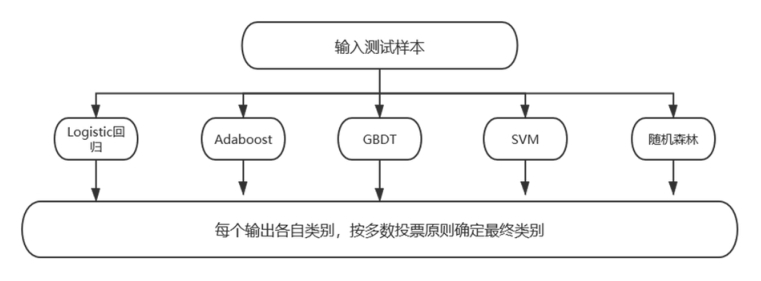
\includegraphics[width=1.0\textwidth,height=0.38\textwidth]{img/1/voting.png} % 图片相对位置
	\caption{Voting 模型图解}
	% \label{fig:figure 3} % 图片标签
\end{figure}

\subsubsection{模型求解}

首先对 5 个基分类进行数据拟合和调参,选取较优参数,得出 5 个基分类器在改数据集上表现,如下表所示:
\begin{table}[!ht]
	\centering
	\caption{基分类器分类效果}
	\begin{tabular}{|l|l|l|l|l|}
		\hline
		分类器       & 测试集准确率 & 训练集准确率 & 综合准确率 & AUC值 \\ \hline
		Logistic回归 & 0.839        & 0.902        & 0.886      & 0.754 \\ \hline
		Adaboost     & 0.903        & 0.913        & 0.911      & 0.822 \\ \hline
		GBDT         & 0.806        & 1            & 0.951      & 0.942 \\ \hline
		SVM          & 0.871        & 0.978        & 0.951      & 0.889 \\ \hline
		随机森林     & 0.871        & 1            & 0.967      & 0.953 \\ \hline
	\end{tabular}
\end{table}

从表 1 可以看出,训练集和测试集效果最接近的为 Adaboost,其余的分类器有程度不一样的过拟合现象。在整体上,Logistic 回归明显略逊一筹,后三个分类器的结果较为接近,主要是三个分类器在训练集上都有良好的表现,而训练集数据占到了整体数据的 7 成。
然而仅从准确率的角度判断分类模型的结果是有失偏颇的,并且本文的目的是,所以本文加入了 AUC 值进行参考。AUC 值为 ROC 曲线覆盖的面积,其含义可以综合的考虑召回率(recall),精确率(precision)和准确率(accuracy)多种指标,一般 AUC 值达到 0.8 以上分类模型可以接受,从这个角度来看,Logistic 回归不符合要求。
因为各个基分类器的分类效果不一样,所以本文选择软投票,依据分类器在整体数据上的综合准确率来判断各基分类器的权重,公式为:
\begin{equation}
	W=\frac{Accuracy_i}{\sum^{5}_{i=1}Accuracy_i}
\end{equation}

软投票分类结果如下表,
\begin{table}[!ht]
	\centering
	\begin{tabular}{c c c c c}
		\hline
		分类器      & 测试集准确率 & 训练集准确率 & 综合准确率 & AUC值 \\ \hline
		Soft Voting & 0.903        & 1            & 0.976      & 0.994 \\ \hline
	\end{tabular}
\end{table}

可以看出,Soft Voting 在分类上的表现十分完美,非常接近完美分类器,说明集成学习算法在此数据集上有着优秀的表现。

\begin{figure}[H]\centering
	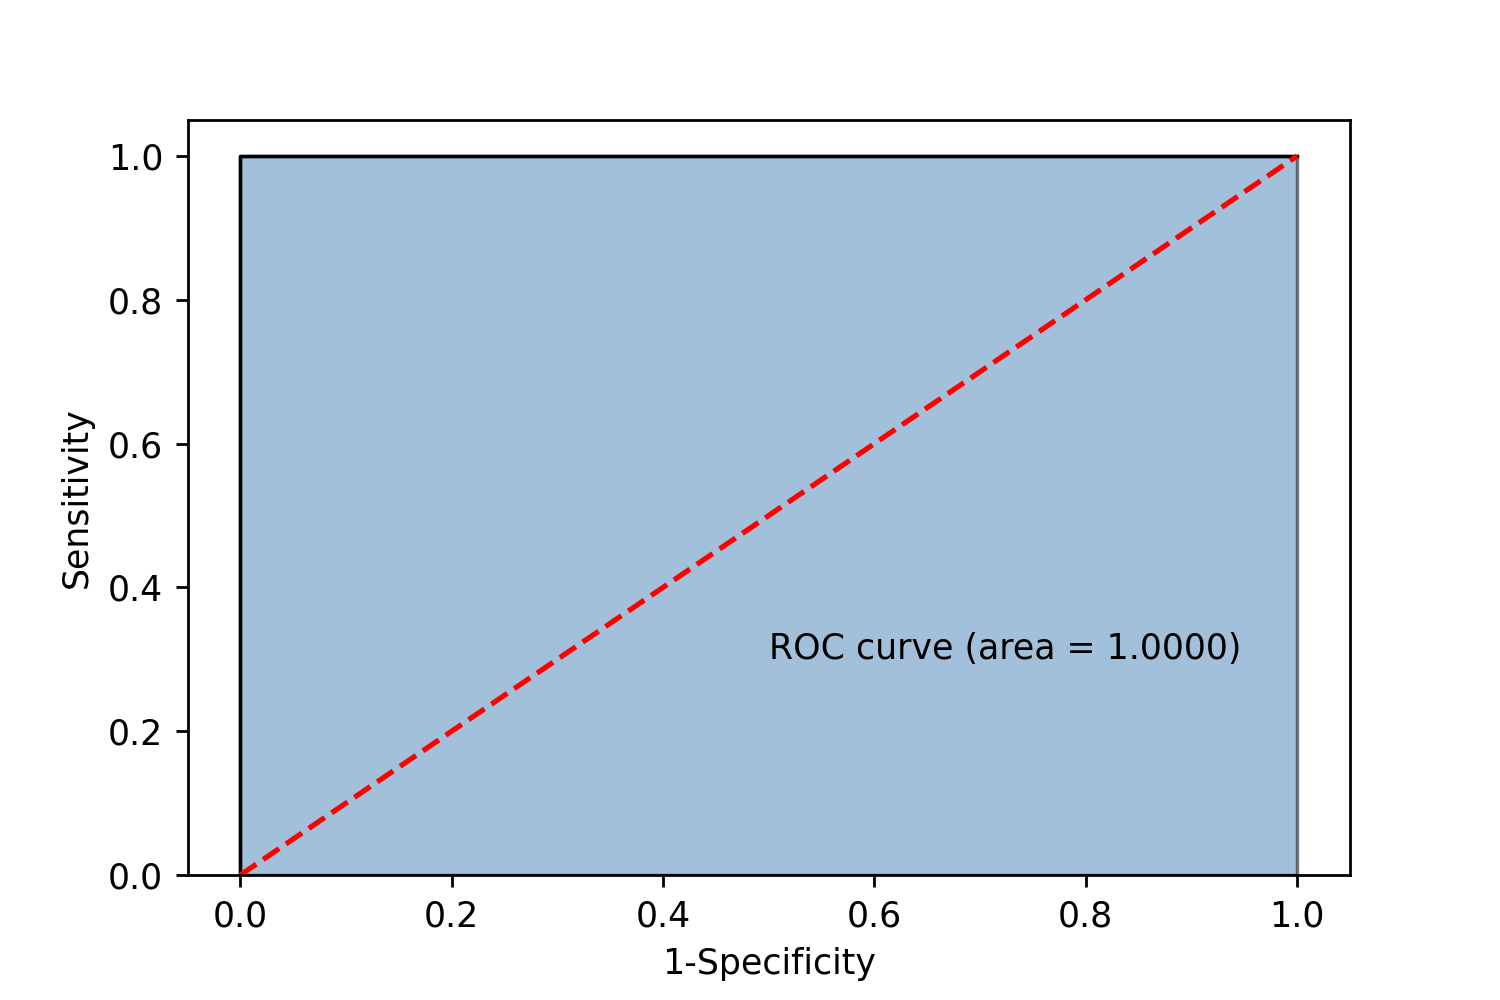
\includegraphics[width=0.8\textwidth,height=0.5\textwidth]{img/1/AUC.png} % 图片相对位置
	\caption{Voting 模型图解}
	% \label{fig:figure 3} % 图片标签
\end{figure}

Voting 模型不仅可以判断出企业是否户违约,并且可以给出企业违约的概率,本文将在后文以此作为对企业的信贷风险的度量。依据信誉评级分类,对不同类别企业的违约风险进行描述性统计分析,表格如下:

\begin{table}[!ht]
	\centering
	\caption{不同信誉评级下违约风险的描述性统计分析}
	\begin{tabular}{c c c c}
		\hline
		A     & B           & C           & D           \\ \hline
		count & 27          & 38          & 34          \\ \hline
		mean  & 0.136353465 & 0.606529877 & 0.581238015 \\ \hline
		std   & 0.095316732 & 0.061405565 & 0.039483599 \\ \hline
		min   & 0.089450606 & 0.564580314 & 0.565384431 \\ \hline
		25\%  & 0.091497276 & 0.569940525 & 0.56725445  \\ \hline
		50\%  & 0.091497276 & 0.571360336 & 0.569940525 \\ \hline
		75\%  & 0.092452513 & 0.670804927 & 0.571360336 \\ \hline
		max   & 0.339357524 & 0.711942814 & 0.70760367  \\ \hline
	\end{tabular}
\end{table}

\subsection{信贷策略多目标规划模型}

\subsubsection{模型分析}

根据假设 2,银行将对信誉评级在 C 及其以上并且之前没有违约记录的的企业发放贷款,即符合条件的企业共有 96 家,其中 A 级企业 27 家,B 级企业 37 家和 C 级企业 32 家。银行的放贷决策需要考虑自身利益,即综合的考虑收益和风险,决定对各级企业的放贷额度和利率优惠,这将自然转化为一个多目标规划问题。

首先,由假设 1 可知银行认为同种信誉评级下的企业的违约风险一直,且在前文
10

中已经求出了每种类别的平均违约风险$\hat \sigma_i $,故由每类企业的$\hat \sigma_i $代表该类信誉评级下企业的违约风险。

\subsubsection{模型建立与求解}

收益目标:银行的目标之一为收益最大化,银行给予企业贷款得到的收益是利息
收益,即
\begin{equation}
	max\sum_{i=1}^3 C_i \cdot I_i \cdot P_i
\end{equation}

风险目标:银行的目标之一为风险最小,如果企业违约,即银行不仅收不回利
息,也收不回本金,所以银行希望最小化损失,即
\begin{equation}
	min\sum_{i=1}^3 C_i \cdot \hat \sigma_i \cdot I_i \cdot P_i \cdot (I_i+1)
\end{equation}

潜在损失目标:银行会因为调高利率,而流失潜在客户,这些流失的客户也对银行造成了潜在损失,银行也希望吸引更多的企业来贷款,可以获得更多的利息收益。由假设 6 可知,已知附件来贷款的企业的数量,通过利率可以算出流失的潜在客户数,即$\frac{C_i \cot Lost(I_i)}{1-Lost(I_i)}$。若流失了一个潜在客户,则银行就失去了贷款从而获得利息的机会,银行希望这笔损失最小,即
\begin{equation}
	\min \sum_{i=1}^3 {\frac{C_i \cot Lost(I_i)}{1-Lost(I_i)}} \cdot I_i \cdot P_i
\end{equation}

查阅资料,我们发现银行有对贷款额度进行分级的实践,不同信用等级的企业能贷的最大贷款和最低利率不同,所以银行应该对信用等级高的企业优先给予贷款,且提供数额较大,利率较低的贷款,以满足银行对收益和风险的追求。本文因此对不同信誉评级的企业贷款的额度和利率的上下限做出规定,以此来规范贷款行为,具体规则如下:

\begin{table}[!ht]
	\centering
	\caption{不同信誉等级下的贷款限制}
	\begin{tabular}{c c c}
		\hline
		信誉评级 & 利率下限 & 贷款额度上限 \\ \hline
		A        & 4\%      & 100          \\ \hline

		B        & 7.5\%    & 70           \\ \hline

		C        & 11\%     & 40           \\ \hline
	\end{tabular}
\end{table}

综上所述,银行在贷款额度为固定数额的约束下(本问定为 5000 万),要使得满足上述三个目标,将上述三个目标转化为单一目标,列式可得:

\begin{equation}
	\min \sum_{i=1}^{3} C_{i}^{*} \bar{\sigma}_{i}^{*} P_{i} *\left(1+I_{i}\right)+I_{i} * P_{i}^{*} \frac{C_{i}^{*} \operatorname{Lost}\left(I_{i}\right)}{1-\operatorname{Lost}\left(I_{i}\right)}-C_{i}{ }^{*} I_{i}{ }^{*} P_{i}
\end{equation}


\begin{equation}
	\text { s.t. }\left\{\begin{array}{l}
		\sum_{i=1}^{3} C_{i}{ }^{*} P_{i}=50000000 \\
		0.04 \leqslant I_{1} \leqslant 0.15        \\
		0.075 \leqslant I_{2} \leqslant 0.15       \\
		0.11 \leqslant I_{3} \leqslant 0.15        \\
		100000 \leqslant P_{1} \leqslant 1000000   \\
		100000 \leqslant P_{2} \leqslant 700000    \\
		100000 \leqslant P_{1} \leqslant 400000
	\end{array}\right.
\end{equation}

运用 SPSS 求解可得:
\begin{equation}
	\begin{array}{c}
		I_{1}=0.0585, I_{2}=0.075, I_{3}=0.11 \\
		P_{1}=999905, P_{2}=535178, P_{3}=100030
	\end{array}
\end{equation}

故对于附件一中队 123 家企业,银行的信贷策略是,对 D 级企业和有违约经历的企业拒绝提供贷款;剩下的企业中,对 A 级企业提供利率为 5.85\%,额度为 999905 元的贷款;对 B 级企业提供利率为 7.5\%,额度为 535178 元的贷款;对 C 级企业提供利率为 11\%,额度为 100030 元的贷款.


\subsection{问题二的求解}
\subsubsection{数据处理}
依据问题一的数据处理方式,进行特征值的提取,最终获取到企业利润、增值税、进销项发票作废率、是否盈亏、下属分公司
等20个特征值,用作训练模型的处理值。需要利用训练模型进等级评估,依据附件的形式,给出A、B、C、D四个信誉等级。
\subsubsection{违约预测}
采用已经训练好的额$Voting$模型,运用所提取的20个特征进行预测,判断这302家无信贷记录企业的违约风险,
判断企业是否会违约。 给出的判断标准为违约风险超过50$\%$,则表示为风险高,不予以贷款。
通过Voting模型的计算最终得到302个违约风险中,有34家企业的违约风险超过了50$\%$,即认为会违约,银行将不会向他们提供贷款。
\subsubsection{信誉分类}
有信贷记录的企业是依据信誉等级来进行确定贷款是否发放,对于这些没有信誉等级的企业则需要对他们进行信誉分级。
通过对特征值的计算,来进行分级,从而确定信贷策略。

本文采用的是$XGboost$模型进行分类,$XGboost$具有较好的分类功能,基于Boosting型的树集成模型。
在梯度提升决策树$GBDT$基础上扩展,能够进行多线程并行计算,通过迭代生成新树,
即可将多个分类性能较低的弱学习器组合为一个准确率较高的强学习器。采用随机森林对字段抽样,将正则项引入损失函数中,
从而防止模型过拟合,并降低模型计算量。

\subsubsection{$XGboost$模型建立}
1、设模型具有$k$个决策树:
\begin{equation}
	\hat{y_i}=\sum_{i = 1}^{k}f_k(x_i),f_k \in F
\end{equation}

其中的$F$表示的为所有映射关系集合,可以得到损失函数为:

\begin{equation}
	L(t)=\sum_{i = 1}^{k}l[y_i,\hat{y}(t-1)_i+f_t(x_i)]+\Omega (f_t)
\end{equation}

$L(t)$为迭代时的目标函数,$n$为样本数量,$I$为损失函数,$\hat{y}(t-1)_i$为迭代模型的预测值,$\Omega (f_t)$为正则项。

2、对$L(t)$进行二阶泰勒展开和移除常数项操:
\begin{equation}
	\tilde{L}(t) \cong \sum_{j=i}^T[(\sum_{i\in I_j}d_i)w_i+\frac{1}{2}(\sum_{i\in I_j}g_i+\lambda )\omega ^2_j]+\gamma N
\end{equation}
上式中,$d_i$为$l$对$\hat{y}(t-1)_i$的一阶导数;$g_i$为对$\hat{y}(t-1)_i$的二阶导数,$N$为叶子节点个数,
$I_j$为每个叶子结点上样本集合,$\omega ^2_j$为每个叶子结点分数的$L_2$模的平方,$\lambda$和$\gamma$
则为比重系数,防止产生过拟合。

通过建立$XGboost$模型对附件2中处理得出的20个特征值进行计算。首先先用第一问的数据进行分类
计算其信誉等级,进行附件1的比对,得出较高的准确率,表明用来分类实为合理。通过分类发现,等级越低
其会违约的概率就越高,其中$D$为均会违约的企业。通过与$Voting$训练模型进行比对,发现训练结果较为
接近,证明了$XGboost$模型的有效性。

如下为利用$XGboost$训练得出的信誉等级:
\begin{table}[H]
	\centering
	\caption{XGboost训练的信誉等级}
	\begin{tabular}{|l|l|l|l|l|l|l|l|}
		\hline
		企业代号 & 信誉等级 & 企业代号 & 信誉等级 & 企业代号 & 信誉等级 & 企业代号 & 信誉等级 \\ \hline
		E124     & 3        & E200     & 3        & E275     & 2        & E350     & 1        \\ \hline
		E125     & 2        & E201     & 1        & E276     & 0        & E351     & 1        \\ \hline
		E126     & 3        & E202     & 2        & E277     & 2        & E352     & 1        \\ \hline
		E127     & 3        & E203     & 0        & E278     & 1        & E353     & 2        \\ \hline
		E128     & 0        & E204     & 0        & E279     & 1        & E354     & 1        \\ \hline
		E129     & 2        & E205     & 2        & E280     & 2        & E355     & 2        \\ \hline
		E130     & 0        & E206     & 0        & E281     & 0        & E356     & 2        \\ \hline
		E131     & 2        & E207     & 2        & E282     & 2        & E357     & 2        \\ \hline
		E132     & 3        & E208     & 3        & E283     & 1        & E358     & 2        \\ \hline
		E133     & 0        & E209     & 0        & E284     & 0        & E359     & 2        \\ \hline
		E134     & 0        & E210     & 0        & E285     & 3        & E360     & 2        \\ \hline
	\end{tabular}
\end{table}

\begin{table}[H]
	\centering
	\begin{tabular}{|l|l|l|l|l|l|l|l|}
		\hline
		企业代号 & 信誉等级 & 企业代号 & 信誉等级 & 企业代号 & 信誉等级 & 企业代号 & 信誉等级 \\ \hline
		E134     & 0        & E210     & 0        & E285     & 3        & E360     & 2        \\ \hline
		E135     & 0        & E211     & 3        & E286     & 1        & E361     & 2        \\ \hline
		E136     & 1        & E212     & 0        & E287     & 0        & E362     & 2        \\ \hline
		E137     & 0        & E213     & 0        & E288     & 3        & E363     & 1        \\ \hline
		E138     & 0        & E214     & 1        & E289     & 0        & E364     & 1        \\ \hline
		E139     & 1        & E215     & 0        & E290     & 0        & E365     & 0        \\ \hline
		E140     & 0        & E216     & 0        & E291     & 0        & E366     & 2        \\ \hline
		E141     & 0        & E217     & 3        & E292     & 1        & E367     & 2        \\ \hline
		E142     & 0        & E218     & 2        & E293     & 2        & E368     & 2        \\ \hline
		E143     & 0        & E219     & 2        & E294     & 3        & E369     & 2        \\ \hline
		E144     & 0        & E220     & 0        & E295     & 0        & E370     & 2        \\ \hline
		E145     & 0        & E221     & 1        & E296     & 1        & E371     & 2        \\ \hline
		E146     & 1        & E222     & 0        & E297     & 2        & E372     & 2        \\ \hline
		E147     & 0        & E223     & 2        & E298     & 2        & E373     & 3        \\ \hline
		E148     & 0        & E224     & 1        & E299     & 1        & E374     & 2        \\ \hline
		E149     & 0        & E225     & 0        & E300     & 0        & E375     & 2        \\ \hline
		E150     & 0        & E226     & 1        & E301     & 0        & E376     & 2        \\ \hline
		E151     & 0        & E227     & 0        & E302     & 0        & E377     & 1        \\ \hline
		E152     & 0        & E228     & 0        & E303     & 0        & E378     & 1        \\ \hline
		E153     & 3        & E229     & 0        & E304     & 1        & E379     & 2        \\ \hline
		E154     & 1        & E230     & 1        & E305     & 2        & E380     & 2        \\ \hline
		E155     & 2        & E231     & 0        & E306     & 3        & E381     & 0        \\ \hline
		E156     & 3        & E232     & 2        & E307     & 1        & E382     & 2        \\ \hline
		E157     & 2        & E233     & 1        & E308     & 1        & E383     & 2        \\ \hline
		E158     & 1        & E234     & 0        & E309     & 3        & E384     & 3        \\ \hline
		E159     & 2        & E235     & 3        & E310     & 1        & E385     & 2        \\ \hline
		E160     & 0        & E236     & 3        & E311     & 0        & E386     & 3        \\ \hline
		E161     & 1        & E237     & 3        & E312     & 1        & E387     & 2        \\ \hline
		E162     & 0        & E238     & 2        & E313     & 0        & E388     & 2        \\ \hline
		E163     & 0        & E239     & 3        & E314     & 0        & E389     & 2        \\ \hline
		E164     & 3        & E240     & 3        & E315     & 0        & E390     & 2        \\ \hline
		E165     & 0        & E241     & 3        & E316     & 3        & E391     & 2        \\ \hline
		E166     & 0        & E242     & 3        & E317     & 1        & E392     & 1        \\ \hline
		E167     & 0        & E243     & 0        & E318     & 2        & E393     & 2        \\ \hline
		E168     & 2        & E244     & 3        & E319     & 2        & E394     & 0        \\ \hline
		E169     & 1        & E245     & 1        & E320     & 2        & E395     & 1        \\ \hline
		E170     & 0        & E246     & 0        & E321     & 1        & E396     & 1        \\ \hline
		E171     & 0        & E247     & 1        & E322     & 1        & E397     & 2        \\ \hline
		E172     & 1        & E248     & 0        & E323     & 2        & E398     & 2        \\ \hline
	\end{tabular}
\end{table}

\begin{table}[H]
	\centering
	\begin{tabular}{|l|l|l|l|l|l|l|l|}
		\hline
		企业代号 & 信誉等级 & 企业代号 & 信誉等级 & 企业代号 & 信誉等级 & 企业代号 & 信誉等级 \\ \hline
		E173     & 2        & E249     & 2        & E324     & 0        & E399     & 2        \\ \hline
		E174     & 1        & E250     & 0        & E325     & 1        & E400     & 2        \\ \hline
		E175     & 0        & E251     & 1        & E326     & 0        & E401     & 1        \\ \hline
		E176     & 0        & E252     & 0        & E327     & 2        & E402     & 2        \\ \hline
		E177     & 0        & E253     & 0        & E328     & 2        & E403     & 2        \\ \hline
		E178     & 1        & E254     & 2        & E329     & 2        & E404     & 3        \\ \hline
		E179     & 0        & E255     & 3        & E330     & 0        & E405     & 2        \\ \hline
		E180     & 0        & E256     & 2        & E331     & 2        & E406     & 2        \\ \hline
		E181     & 0        & E257     & 2        & E332     & 2        & E407     & 2        \\ \hline
		E182     & 1        & E258     & 0        & E333     & 0        & E408     & 1        \\ \hline
		E183     & 0        & E259     & 2        & E334     & 2        & E409     & 2        \\ \hline
		E184     & 0        & E260     & 0        & E335     & 2        & E410     & 2        \\ \hline
		E185     & 1        & E261     & 0        & E336     & 2        & E411     & 1        \\ \hline
		E186     & 0        & E262     & 1        & E337     & 2        & E412     & 2        \\ \hline
		E187     & 3        & E263     & 1        & E338     & 2        & E413     & 1        \\ \hline
		E188     & 0        & E264     & 3        & E339     & 2        & E414     & 2        \\ \hline
		E189     & 1        & E265     & 1        & E340     & 2        & E415     & 2        \\ \hline
		E190     & 1        & E266     & 1        & E341     & 2        & E416     & 2        \\ \hline
		E191     & 1        & E267     & 2        & E342     & 0        & E417     & 1        \\ \hline
		E192     & 0        & E268     & 1        & E343     & 2        & E418     & 2        \\ \hline
		E193     & 2        & E269     & 0        & E344     & 2        & E419     & 1        \\ \hline
		E194     & 0        & E270     & 3        & E345     & 1        & E420     & 1        \\ \hline
		E195     & 0        & E271     & 0        & E346     & 3        & E421     & 2        \\ \hline
		E196     & 0        & E272     & 3        & E347     & 1        & E422     & 2        \\ \hline
		E197     & 0        & E273     & 2        & E348     & 2        & E423     & 2        \\ \hline
		E198     & 0        & E274     & 2        & E349     & 2        & E424     & 2        \\ \hline
	\end{tabular}
\end{table}

由$Voting$模型训练的违约风险表格参见附件。

\subsubsection{信贷策略}
依据$XGboost$算法对302家企业进行了信誉等级分类,得出由268家企业是符合放贷标准之一的
信誉等级合格。依据分类出的$A$、$B$、$C$三类企业,参照第一问的信贷策略方式对不同信誉
等级的贷款限制方式,得出如下的目标规划模型:
\begin{equation}
	\min \sum_{n = 1}^{3}C_i\sigma_n P_n (1+I_n)+I_n P_n \frac{C_n Lost(I_n)}{Lost(I_n)}-C_n I_n P_n
\end{equation}

\newpage

限制条件为:
\[\left\{\begin{array}{lllll}
		\sum_{n = 1}^{3}C_n \sigma_n P_n = 10^7 \\
		0.04 \le I_1 \le 0.15                   \\
		0.075 \le I_2 \le 0.15                  \\
		0.11 \le I_3 \le 0.15                   \\
		10^5 \le P_1 \le 10^6                   \\
		10^5 \le P_2 \le 7*10^5                 \\
		10^5 \le P_1 \le 4*10^5                 \\
	\end{array}\right. \]

通过对目标规划进行求解得出,对D级企业和有违约经历的企业拒绝提供贷款;也就是
为$A$、$B$、$C$三类会提供贷款服务,根据等级不同,利率和额度也不同。如下为信誉等级不同
的贷款策略

1、对A级企业提供利率为 7.05$\%$,额度为999717元的贷款;

2、对B 级企业提供利率为7.52$\%$,额度为260320元的贷款;

3、对C级企业提供利率为 11.01$\%$,额度为 100048 元的贷款。
\subsection{问题三的求解}
\subsubsection{数据处理}
第三问的分析评价中加入各种突发情况因素的判断,需要考虑各种突发因素对企业贷款能力的影响,
例如疫情和自然灾害等情况。在第三问中需要加入对新冠疫情对实体企业的冲击的判断条件,
合理估计疫情对企业的影响情况。考虑到2020数据只有一二月,则对应同年增长率计算时也考虑一二月的数据。
根据题目,提取出如下四个主要的特征值:企业盈利状况、对比同年增长率、
废票占比增长率、交易数量变动率。

\textbf{1、企业盈利状况}

在第三问中需要加入对新冠疫情对实体企业的鉴于疫情对于企业的影响情况,
我们主要对企业中有2020年之后存在销项和进项的进行研究。
采用销项金额减去进项金额得到的数值即是盈利的情况。
当$\Delta \ge 0$时,公司为盈利状态,令$Rev$为1;当$\Delta = 0$时,则代表没有交易产生,
令$Rev$为0;当$\Delta \le 0$时,企业处于亏损,令$Rev$为-1。

\textbf{2、对比同年增长率}

这用来主要反映新冠疫情对企业2020年盈利的冲击,对比2019年会有什么变化,主观的反映了疫情
这一突发因素对企业盈利能力的干扰。其值为20年利润减去19年利润比上19年的利润。
\begin{equation}
	Profit = \frac{Pf(20020,i)-Pf(2019,i)}{Pf(2019,i)},i=(1,2)
\end{equation}

\textbf{3、废票占比增长率}

废票为交易活动开具发票后,因故取消了该项交易,而作废的发票,废票变动情况能够反映疫情到来
对交易活动的影响,会使得取消交易的情况增多还是减少,通过与2019数据的对比来体现这一特征值的特性。
\begin{equation}
	Void = \frac{V(20020,i)-V(2019,i)}{V(2019,i)},i=(1,2)
\end{equation}

\textbf{4、交易数量变动率}

考虑到企业的交易数量也是对企业整体规模的一个考察,本问中是提取2019和2020年一月和二月期间
企业的交易数量,依据发票单号指标来筛选唯一企业的数量,从而求解变化率。

\begin{equation}
	Trade = \frac{Tra(20020,i)-Tra(2019,i)}{Tra(2019,i)},i=(1,2)
\end{equation}


\subsubsection{聚类模型的建立}

第三问的分析评价中加入各种突发情况因素的判断,需要考虑各种突发因素对企业贷款能力的影响,
例如疫情和自然灾害等情况。在第三问中需要加入对新冠疫情对实体企业的冲击的判断条件,
合理估计疫情对企业的影响情况。

综合各种主流媒体的新闻信息,我们判断新冠疫情会对实体企业产生较大的冲击,
可能会导致企业存在违约风险。鉴于新冠疫情的影响程度对于不同的行业和企业会造成不一样的影响情况,
所以我们需要分类进行考虑。该风险属于一种系统风险,存在不可避免的情况,
各个企业所受到的打击程度不一。

在附件提供的数据中,有多家企业可以归为一类行业。
因为地理和发展情况等因素的影响,不同的企业对于疫情的应对情况也有不同,
可能存在扭亏为盈或者亏损的情况出现,即各个企业都有可能由于突发情况有各种不同的境遇。
在数据上可以表现的特征是利润的发展情况、同期增长比率、废票的占比情况、上下游的供求企业的数量的变化等。

采用聚类模型的好处是,未知企业的收突发因素干扰后的违约因素为多少,在问题二中已经对302家
无信贷记录的企业进行了信誉等级分析,在已有的数据基础上,加入风险系数这个数据值来反映
新冠疫情对企业的影响,也通过新的聚类分析大类来重新指定新的信贷策略,在分类这个基础上,
本题更适合采用聚类分析的建模方法。

\textbf{构建步骤}

将上面计算的4种特征值作为系统聚类的依据。系统聚类的流程是:1、将每一个样本都分为一类;2、计算子类与子类之间的距离,逐渐将所有的子类合并为一个大类。
系统聚类算法的流程如下图所示。
\begin{figure}[H]\centering
	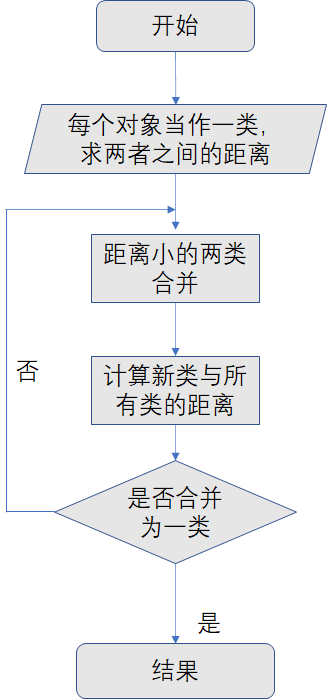
\includegraphics[width=0.4\textwidth,height=0.72\textwidth]{img/3/Clustering.png} % 图片相对位置
	\caption{Clustering}
	\label{fig:figure 2} % 图片标签
\end{figure}

通过python的sklearn库进行聚类,为了确定聚类类别$K$,本文使用肘部法以及轮廓系数进行判断,下面是对应的折线图:

\begin{figure}[H]\centering
	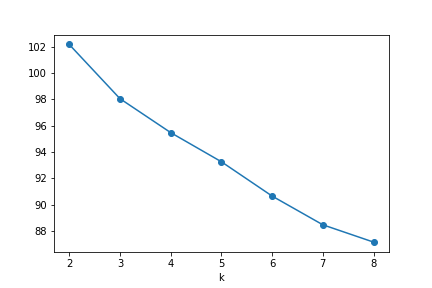
\includegraphics[width=0.8\textwidth,height=0.5\textwidth]{img/3/1.png} % 图片相对位置
	\caption{肘部法折线图}
	% \label{fig:figure 2} % 图片标签
\end{figure}

\begin{figure}[H]\centering
	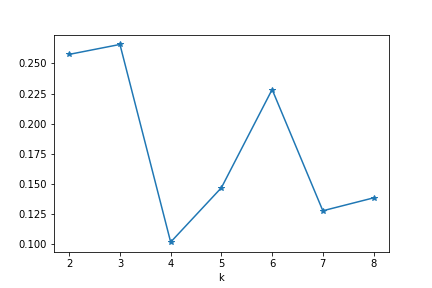
\includegraphics[width=0.8\textwidth,height=0.5\textwidth]{img/3/2.png} % 图片相对位置
	\caption{轮廓系数折线图}
	% \label{fig:figure 2} % 图片标签
\end{figure}

根据聚合系数折线图,可以看出,令$K$=2,聚类效果最好。得出聚类结果后,对聚类的结果分别进行描述性统计分析,可得下面两表。

\newpage
\begin{center}
	\begin{longtable}{|c|c|c|c|}
		\caption{类别一描述}
		\label{tab:aaa}                                                 \\
		\hline
		count                      & mean & min          & max          \\ \hline
		销-进金额                  & 56   & 66835446.05  & -36469795.66 \\ \hline
		增值税                     & 56   & 5104104.041  & 0            \\ \hline
		持续一年期的交易企业个数   & 56   & 322.4285714  & 9            \\ \hline
		持续二年期的交易企业个数   & 56   & 53.78571429  & 0            \\ \hline
		持续三年期的交易企业个数   & 56   & 20.91071429  & 0            \\ \hline
		持续四年前的交易企业个数   & 56   & 0            & 0            \\ \hline
		持续一年期的交易企业个数.1 & 56   & 173.8035714  & 1            \\ \hline
		持续二年期的交易企业个数.1 & 56   & 50.28571429  & 0            \\ \hline
		持续三年期的交易企业个数.1 & 56   & 29.05357143  & 0            \\ \hline
		持续四年前的交易企业个数.1 & 56   & 0            & 0            \\ \hline
		进项发票的作废比例         & 56   & 0.03971703   & 0            \\ \hline
		销项发票的作废比例         & 56   & 0.181496119  & 0.009041591  \\ \hline
		绝对数变化                 & 56   & -3208523.846 & -99670948.43 \\ \hline
		比例变化                   & 56   & 2.575802002  & -3.149295957 \\ \hline
		是否扭亏为1                & 56   & 0.053571429  & 0            \\ \hline
		是否变为-1                 & 56   & 0.071428571  & 0            \\ \hline
		下属部门                   & 56   & 0            & 0            \\ \hline
		分公司                     & 56   & 0            & 0            \\ \hline
		公司                       & 56   & 0            & 0            \\ \hline
		个体经营                   & 56   & 1            & 1            \\ \hline
		是否违约                   & 56   & 0.910714286  & 0            \\ \hline
		违约风险                   & 56   & 0.524032236  & 0.48632597   \\ \hline
		信誉评级                   & 56   & 2.446428571  & 0            \\ \hline
		一月进项总额               & 56   & 0            & 0            \\ \hline
		一月销项总额               & 56   & 0            & 0            \\ \hline
		二月进项总额               & 56   & 0            & 0            \\ \hline
		二月销项总额               & 56   & 0            & 0            \\ \hline
		一月1情况                  & 56   & 0            & 0            \\ \hline
		二月1情况                  & 56   & 0            & 0            \\ \hline
		一月状态                   & 56   & 0            & 0            \\ \hline
		二月状态                   & 56   & 0            & 0            \\ \hline
		较2019一月增长率           & 56   & -0.982142857 & -1           \\ \hline
		较2019二月增长率           & 56   & -4.576230048 & -201.8212513 \\ \hline
		一月废票占比变动           & 56   & -0.875       & -1           \\ \hline
		二月废票占比变动           & 56   & -0.589285714 & -1           \\ \hline
		一月交易企业数量变动率     & 56   & -0.946428571 & -1           \\ \hline
		二月交易企业数量变动率     & 56   & -0.982142857 & -1           \\ \hline
		小                         & 56   & 0.678571429  & 0            \\ \hline
		中                         & 56   & 0.160714286  & 0            \\ \hline
		微                         & 56   & 0            & 0            \\ \hline
		行业评分                   & 56   & 2            & 2            \\ \hline
		聚类类别                   & 56   & 1            & 1            \\ \hline
	\end{longtable}
\end{center}



\begin{center}
	\begin{longtable}{|c|c|c|c|}
		\caption{类别二描述}
		\label{tab:aaaa}                                                \\
		\hline
		count                      & mean & min          & max          \\ \hline
		销-进金额                  & 245  & 17751366.59  & -85467299.95 \\ \hline
		增值税                     & 245  & 1348445.556  & -2098294.08  \\ \hline
		持续一年期的交易企业个数   & 245  & 163.3836735  & 0            \\ \hline
		持续二年期的交易企业个数   & 245  & 34.94285714  & 0            \\ \hline
		持续三年期的交易企业个数   & 245  & 12.63673469  & 0            \\ \hline
		持续四年前的交易企业个数   & 245  & 2.808163265  & 0            \\ \hline
		持续一年期的交易企业个数.1 & 245  & 122.3959184  & 0            \\ \hline
		持续二年期的交易企业个数.1 & 245  & 17.77959184  & 0            \\ \hline
		持续三年期的交易企业个数.1 & 245  & 7.612244898  & 0            \\ \hline
		持续四年前的交易企业个数.1 & 245  & 2.195918367  & 0            \\ \hline
		进项发票的作废比例         & 245  & 0.029965815  & 0            \\ \hline
		销项发票的作废比例         & 245  & 0.112597305  & 0            \\ \hline
		绝对数变化                 & 245  & 3556640.925  & -36622527.16 \\ \hline
		比例变化                   & 245  & -0.006973823 & -469.7670429 \\ \hline
		是否扭亏为1                & 245  & 0.102040816  & 0            \\ \hline
		是否变为-1                 & 245  & 0.06122449   & 0            \\ \hline
		下属部门                   & 245  & 0.06122449   & 0            \\ \hline
		分公司                     & 245  & 0.020408163  & 0            \\ \hline
		公司                       & 245  & 0.86122449   & 0            \\ \hline
		个体经营                   & 245  & 0            & 0            \\ \hline
		是否违约                   & 245  & 0            & 0            \\ \hline
		违约风险                   & 245  & 0.105497714  & 0.083587265  \\ \hline
		信誉评级                   & 245  & 0.987755102  & 0            \\ \hline
		一月进项总额               & 245  & 391348.5854  & -2629.47     \\ \hline
		一月销项总额               & 245  & 778081.855   & -15265.72    \\ \hline
		二月进项总额               & 245  & 11549.72127  & 0            \\ \hline
		二月销项总额               & 245  & 41640.93073  & 0            \\ \hline
		一月1情况                  & 245  & 386733.2696  & -3590298.7   \\ \hline
		二月1情况                  & 245  & 30091.20947  & -919791.78   \\ \hline
		一月状态                   & 245  & 0.310204082  & -1           \\ \hline
		二月状态                   & 245  & -0.081632653 & -1           \\ \hline
		较2019一月增长率           & 245  & -0.494989788 & -235.9578557 \\ \hline
		较2019二月增长率           & 245  & 0.723062694  & -235.9578557 \\ \hline
		一月废票占比变动           & 245  & -0.178098333 & -1           \\ \hline
		二月废票占比变动           & 245  & 0.00391861   & -1           \\ \hline
		一月交易企业数量变动率     & 245  & -0.346759541 & -1           \\ \hline
		二月交易企业数量变动率     & 245  & -0.712798864 & -1           \\ \hline
		小                         & 245  & 0.510204082  & 0            \\ \hline
		中                         & 245  & 0.020408163  & 0            \\ \hline
		微                         & 245  & 0            & 0            \\ \hline
		行业评分                   & 245  & 7.481632653  & 4            \\ \hline
		聚类类别                   & 245  & 2            & 2            \\ \hline
	\end{longtable}
\end{center}


综合上三表数据,类别1的企业大部分为2020年依然盈利或者不盈不亏;
平均$Void_{ij}$较小,$Trade_{ij}$大部分为正且数值较大,说明疫情对于这些企业的影响较小,供求关系稳定甚至仍有盈利;
类别2 的企业大部分为亏损,特征值$Void_{ij}$和$Trade_{ij}$都比类别1要表现更差;类别3的企业有4个,全部为高风险的企业。

根据以上聚类出的三类行业的表现,本文设置其对应的风险乘数为:$Q_1=1$,$Q_2=1.5$,$Q_3=2$


\subsubsection{信贷策略}
附件2中及本文将企业依据信誉评级分为4 类,在建立模型的过程中根据疫情对企业的影响将企业分为3类,
同时将违约和D 级企业不放贷款且聚类结果的类别3全为D级企业。将数据分为6类,
根据聚类结果建立一个新的评价分级体系,记为$A_1$,$A_2$,$B_1$,$B_2$,$C_1$,$C_2$,。
将风险乘数$Q_i$加入信贷目标规划模型,调整企业风险,建立调整后的多目标规划模型如下:
\begin{equation}
	\min \sum_{n = 1}^{3}\sum_{m}C_i(1+Q_m)\overline{\sigma }_n P_n (1+I_m)+I_n P_n \frac{C_n Lost(I_n)}{1-Lost(I_n)}-C_n I_n P_n
\end{equation}

限制条件为:
\[\left\{\begin{array}{lllll}
		\sum_{n = 1}^{6}C_n  P_n = 10^7 \\
		0.04 \le I_1 \le 0.15           \\
		0.058 \le I_2 \le 0.15          \\
		0.076 \le I_3 \le 0.15          \\
		0.094 \le I_4 \le 0.15          \\
		0.112 \le I_5 \le 0.15          \\
		0.13 \le I_6 \le 0.15           \\
		10^5 \le P_1 \le 10^6           \\
		10^5 \le P_2 \le 8.5*10^5       \\
		10^5 \le P_3 \le 7*10^5         \\
		10^5 \le P_4 \le 5.5*10^5       \\
		10^5 \le P_5 \le 4*10^5         \\
		10^5 \le P_6 \le 2.5*10^5       \\
	\end{array}\right. \]

计算得出如下结果:

\begin{table}[!ht]
	\centering
	\caption{借贷方案}
	\begin{tabular}{||c c c c ||}

		\hline
		企业类别 & 数量 & 利率      & 金额   \\ [0.5ex]
		\hline
		$A_1$    & 54   & 7.60$\%$  & 999988 \\
		\hline
		$A_2$    & 9    & 6.25$\%$  & 849863 \\
		\hline
		$B_1$    & 82   & 11.20$\%$ & 317698 \\
		\hline
		$B_2$    & 21   & 9.40$\%$  & 100017 \\
		\hline
		$C_1$    & 87   & 11.20$\%$ & 100002 \\
		\hline
		$C_2$    & 15   & 13.00$\%$ & 100006 \\
		\hline
	\end{tabular}
\end{table}


\section{模型分析}
\subsection{优点}

1、综合考量了企业自身能力和多方因素,从而提取了具有相特征性的特征值数据,较为全面的考虑了问题。

2、使用了多种算法和模型,采用强分类器,效果良好,以及$Voting$集成算法,所得出的结果准确较高,
训练求解的结果可信度同样也很高。

3、考虑信贷策略时,综合考虑了多目标规划,在所提取特征值的基础上,加入了风险系数以及信誉等级
的分类,使得模型更加贴合实际情况。

4、采用的聚类模型在处理突发因素所带来的影响时,得出的轮廓系数接近1,聚类效果好。

\subsection{缺点}
1、数据不够充分,考虑疫情对评估影响时只采用了两年分别四个月的数据,数据不够充分,说服性不足。

2、考虑突发情况时没有充分考虑对企业大类的影响,只考虑了新冠疫情,因素不够多。

3、特征值提取过多,且有的特征值其特征性不明显,作用不大。

4、未对企业进行行业的分类,考虑行业受因素的影响以及总体社会的受干扰因素。

\subsection{改进}
1、可以尝试采用修正因子量化分析的方法来对整体企业进行新的风险评估。

2、可以将企业依据行业进行分类,更好的考虑行业的整体受突发因素影响。


% %引用
% \clearpage
% \bibliographystyle{plain}
% \bibliography{ref}%ref指向自己创建的ref.bib
% % IoU\cite{zheng2020distance}
% \clearpage

\newpage

\section{参考文献}
 [1] 王晓燕.上市民营企业信用风险度量方法研究[D].山东大学,2020.

[2] 刘琪.小额贷款公司个人贷款信用风险评估研究[D].扬州大学,2011.

[3] 顾洲一.基于 XGBoost 模型的银行信贷高风险客户识别研究——以我国 Y 银行


\newpage

\subsection{第二问最终分类结果}

\begin{center}
	\begin{longtable}{|c|c|c|}
		\caption{第二问预测结果}
		\label{tab:dasfa}              \\
		\hline
		企业代号 & 是否违约 & 信誉评级 \\ \hline
		E124     & 是       & D        \\ \hline
		E125     & 否       & C        \\ \hline
		E126     & 是       & D        \\ \hline
		E127     & 是       & D        \\ \hline
		E128     & 是       & A        \\ \hline
		E129     & 否       & C        \\ \hline
		E130     & 是       & A        \\ \hline
		E131     & 否       & C        \\ \hline
		E132     & 是       & D        \\ \hline
		E133     & 是       & A        \\ \hline
		E134     & 否       & A        \\ \hline
		E135     & 否       & A        \\ \hline
		E136     & 否       & B        \\ \hline
		E137     & 否       & A        \\ \hline
		E138     & 是       & A        \\ \hline
		E139     & 是       & B        \\ \hline
		E140     & 否       & A        \\ \hline
		E141     & 否       & A        \\ \hline
		E142     & 否       & A        \\ \hline
		E143     & 否       & A        \\ \hline
		E144     & 否       & A        \\ \hline
		E145     & 否       & A        \\ \hline
		E146     & 否       & B        \\ \hline
		E147     & 否       & A        \\ \hline
		E148     & 否       & A        \\ \hline
		E149     & 否       & A        \\ \hline
		E150     & 否       & A        \\ \hline
		E151     & 否       & A        \\ \hline
		E152     & 否       & A        \\ \hline
		E153     & 是       & D        \\ \hline
		E154     & 否       & B        \\ \hline
		E155     & 是       & C        \\ \hline
		E156     & 是       & D        \\ \hline
		E157     & 否       & C        \\ \hline
		E158     & 否       & B        \\ \hline
		E159     & 是       & C        \\ \hline
		E160     & 否       & A        \\ \hline
		E161     & 否       & B        \\ \hline
		E162     & 否       & A        \\ \hline
		E163     & 否       & A        \\ \hline
		E164     & 是       & D        \\ \hline
		E165     & 否       & A        \\ \hline
		E166     & 否       & A        \\ \hline
		E167     & 否       & A        \\ \hline
		E168     & 否       & C        \\ \hline
		E169     & 否       & B        \\ \hline
		E170     & 否       & A        \\ \hline
		E171     & 否       & A        \\ \hline
		E172     & 否       & B        \\ \hline
		E173     & 否       & C        \\ \hline
		E174     & 否       & B        \\ \hline
		E175     & 否       & A        \\ \hline
		E176     & 否       & A        \\ \hline
		E177     & 否       & A        \\ \hline
		E178     & 否       & B        \\ \hline
		E179     & 否       & A        \\ \hline
		E180     & 否       & A        \\ \hline
		E181     & 否       & A        \\ \hline
		E182     & 否       & B        \\ \hline
		E183     & 否       & A        \\ \hline
		E184     & 否       & A        \\ \hline
		E185     & 否       & B        \\ \hline
		E186     & 否       & A        \\ \hline
		E187     & 是       & D        \\ \hline
		E188     & 否       & A        \\ \hline
		E189     & 否       & B        \\ \hline
		E190     & 否       & B        \\ \hline
		E191     & 否       & B        \\ \hline
		E192     & 否       & A        \\ \hline
		E193     & 否       & C        \\ \hline
		E194     & 否       & A        \\ \hline
		E195     & 否       & A        \\ \hline
		E196     & 否       & A        \\ \hline
		E197     & 否       & A        \\ \hline
		E198     & 否       & A        \\ \hline
		E199     & 否       & A        \\ \hline
		E200     & 是       & D        \\ \hline
		E201     & 否       & B        \\ \hline
		E202     & 是       & C        \\ \hline
		E203     & 否       & A        \\ \hline
		E204     & 否       & A        \\ \hline
		E205     & 是       & C        \\ \hline
		E206     & 否       & A        \\ \hline
		E207     & 是       & C        \\ \hline
		E208     & 是       & D        \\ \hline
		E209     & 否       & A        \\ \hline
		E210     & 否       & A        \\ \hline
		E211     & 是       & D        \\ \hline
		E212     & 否       & A        \\ \hline
		E213     & 否       & A        \\ \hline
		E214     & 否       & B        \\ \hline
		E215     & 否       & A        \\ \hline
		E216     & 否       & A        \\ \hline
		E217     & 是       & D        \\ \hline
		E218     & 否       & C        \\ \hline
		E219     & 否       & C        \\ \hline
		E220     & 否       & A        \\ \hline
		E221     & 否       & B        \\ \hline
		E222     & 否       & A        \\ \hline
		E223     & 否       & C        \\ \hline
		E224     & 否       & B        \\ \hline
		E225     & 否       & A        \\ \hline
		E226     & 否       & B        \\ \hline
		E227     & 否       & A        \\ \hline
		E228     & 否       & A        \\ \hline
		E229     & 否       & A        \\ \hline
		E230     & 否       & B        \\ \hline
		E231     & 否       & A        \\ \hline
		E232     & 否       & C        \\ \hline
		E233     & 否       & B        \\ \hline
		E234     & 否       & A        \\ \hline
		E235     & 是       & D        \\ \hline
		E236     & 是       & D        \\ \hline
		E237     & 是       & D        \\ \hline
		E238     & 否       & C        \\ \hline
		E239     & 是       & D        \\ \hline
		E240     & 是       & D        \\ \hline
		E241     & 是       & D        \\ \hline
		E242     & 是       & D        \\ \hline
		E243     & 否       & A        \\ \hline
		E244     & 是       & D        \\ \hline
		E245     & 否       & B        \\ \hline
		E246     & 否       & A        \\ \hline
		E247     & 否       & B        \\ \hline
		E248     & 否       & A        \\ \hline
		E249     & 否       & C        \\ \hline
		E250     & 否       & A        \\ \hline
		E251     & 否       & B        \\ \hline
		E252     & 否       & A        \\ \hline
		E253     & 否       & A        \\ \hline
		E254     & 否       & C        \\ \hline
		E255     & 是       & D        \\ \hline
		E256     & 否       & C        \\ \hline
		E257     & 否       & C        \\ \hline
		E258     & 否       & A        \\ \hline
		E259     & 否       & C        \\ \hline
		E260     & 否       & A        \\ \hline
		E261     & 否       & A        \\ \hline
		E262     & 是       & B        \\ \hline
		E263     & 否       & B        \\ \hline
		E264     & 是       & D        \\ \hline
		E265     & 否       & B        \\ \hline
		E266     & 否       & B        \\ \hline
		E267     & 否       & C        \\ \hline
		E268     & 否       & B        \\ \hline
		E269     & 否       & A        \\ \hline
		E270     & 是       & D        \\ \hline
		E271     & 否       & A        \\ \hline
		E272     & 是       & D        \\ \hline
		E273     & 是       & C        \\ \hline
		E274     & 否       & C        \\ \hline
		E275     & 否       & C        \\ \hline
		E276     & 否       & A        \\ \hline
		E277     & 否       & C        \\ \hline
		E278     & 否       & B        \\ \hline
		E279     & 否       & B        \\ \hline
		E280     & 是       & C        \\ \hline
		E281     & 否       & A        \\ \hline
		E282     & 否       & C        \\ \hline
		E283     & 否       & B        \\ \hline
		E284     & 否       & A        \\ \hline
		E285     & 是       & D        \\ \hline
		E286     & 否       & B        \\ \hline
		E287     & 否       & A        \\ \hline
		E288     & 是       & D        \\ \hline
		E289     & 否       & A        \\ \hline
		E290     & 否       & A        \\ \hline
		E291     & 否       & A        \\ \hline
		E292     & 否       & B        \\ \hline
		E293     & 否       & C        \\ \hline
		E294     & 是       & D        \\ \hline
		E295     & 否       & A        \\ \hline
		E296     & 否       & B        \\ \hline
		E297     & 否       & C        \\ \hline
		E298     & 否       & C        \\ \hline
		E299     & 否       & B        \\ \hline
		E300     & 否       & A        \\ \hline
		E301     & 否       & A        \\ \hline
		E302     & 否       & A        \\ \hline
		E303     & 否       & A        \\ \hline
		E304     & 否       & B        \\ \hline
		E305     & 否       & C        \\ \hline
		E306     & 是       & D        \\ \hline
		E307     & 否       & B        \\ \hline
		E308     & 否       & B        \\ \hline
		E309     & 是       & D        \\ \hline
		E310     & 否       & B        \\ \hline
		E311     & 否       & A        \\ \hline
		E312     & 否       & B        \\ \hline
		E313     & 否       & A        \\ \hline
		E314     & 否       & A        \\ \hline
		E315     & 否       & A        \\ \hline
		E316     & 是       & D        \\ \hline
		E317     & 否       & B        \\ \hline
		E318     & 否       & C        \\ \hline
		E319     & 是       & C        \\ \hline
		E320     & 否       & C        \\ \hline
		E321     & 否       & B        \\ \hline
		E322     & 否       & B        \\ \hline
		E323     & 否       & C        \\ \hline
		E324     & 否       & A        \\ \hline
		E325     & 否       & B        \\ \hline
		E326     & 否       & A        \\ \hline
		E327     & 是       & C        \\ \hline
		E328     & 否       & C        \\ \hline
		E329     & 否       & C        \\ \hline
		E330     & 否       & A        \\ \hline
		E331     & 否       & C        \\ \hline
		E332     & 否       & C        \\ \hline
		E333     & 否       & A        \\ \hline
		E334     & 否       & C        \\ \hline
		E335     & 否       & C        \\ \hline
		E336     & 否       & C        \\ \hline
		E337     & 是       & C        \\ \hline
		E338     & 否       & C        \\ \hline
		E339     & 否       & C        \\ \hline
		E340     & 否       & C        \\ \hline
		E341     & 否       & C        \\ \hline
		E342     & 否       & A        \\ \hline
		E343     & 否       & C        \\ \hline
		E344     & 否       & C        \\ \hline
		E345     & 否       & B        \\ \hline
		E346     & 是       & D        \\ \hline
		E347     & 否       & B        \\ \hline
		E348     & 否       & C        \\ \hline
		E349     & 否       & C        \\ \hline
		E350     & 否       & B        \\ \hline
		E351     & 否       & B        \\ \hline
		E352     & 否       & B        \\ \hline
		E353     & 否       & C        \\ \hline
		E354     & 否       & B        \\ \hline
		E355     & 否       & C        \\ \hline
		E356     & 否       & C        \\ \hline
		E357     & 否       & C        \\ \hline
		E358     & 否       & C        \\ \hline
		E359     & 否       & C        \\ \hline
		E360     & 否       & C        \\ \hline
		E361     & 否       & C        \\ \hline
		E362     & 否       & C        \\ \hline
		E363     & 否       & B        \\ \hline
		E364     & 否       & B        \\ \hline
		E365     & 否       & A        \\ \hline
		E366     & 否       & C        \\ \hline
		E367     & 否       & C        \\ \hline
		E368     & 否       & C        \\ \hline
		E369     & 否       & C        \\ \hline
		E370     & 否       & C        \\ \hline
		E371     & 否       & C        \\ \hline
		E372     & 否       & C        \\ \hline
		E373     & 是       & D        \\ \hline
		E374     & 否       & C        \\ \hline
		E375     & 否       & C        \\ \hline
		E376     & 否       & C        \\ \hline
		E377     & 否       & B        \\ \hline
		E378     & 否       & B        \\ \hline
		E379     & 否       & C        \\ \hline
		E380     & 否       & C        \\ \hline
		E381     & 否       & A        \\ \hline
		E382     & 否       & C        \\ \hline
		E383     & 否       & C        \\ \hline
		E384     & 是       & D        \\ \hline
		E385     & 否       & C        \\ \hline
		E386     & 是       & D        \\ \hline
		E387     & 否       & C        \\ \hline
		E388     & 否       & C        \\ \hline
		E389     & 否       & C        \\ \hline
		E390     & 否       & C        \\ \hline
		E391     & 否       & C        \\ \hline
		E392     & 否       & B        \\ \hline
		E393     & 否       & C        \\ \hline
		E394     & 否       & A        \\ \hline
		E395     & 否       & B        \\ \hline
		E396     & 否       & B        \\ \hline
		E397     & 否       & C        \\ \hline
		E398     & 否       & C        \\ \hline
		E399     & 否       & C        \\ \hline
		E400     & 否       & C        \\ \hline
		E401     & 否       & B        \\ \hline
		E402     & 否       & C        \\ \hline
		E403     & 否       & C        \\ \hline
		E404     & 是       & D        \\ \hline
		E405     & 否       & C        \\ \hline
		E406     & 否       & C        \\ \hline
		E407     & 否       & C        \\ \hline
		E408     & 否       & B        \\ \hline
		E409     & 否       & C        \\ \hline
		E410     & 否       & C        \\ \hline
		E411     & 否       & B        \\ \hline
		E412     & 否       & C        \\ \hline
		E413     & 否       & B        \\ \hline
		E414     & 否       & C        \\ \hline
		E415     & 否       & C        \\ \hline
		E416     & 否       & C        \\ \hline
		E417     & 否       & B        \\ \hline
		E418     & 否       & C        \\ \hline
		E419     & 否       & B        \\ \hline
		E420     & 否       & B        \\ \hline
		E421     & 否       & C        \\ \hline
		E422     & 否       & C        \\ \hline
		E423     & 否       & C        \\ \hline
		E424     & 否       & C        \\ \hline
	\end{longtable}
\end{center}

\newpage

\subsection{代码}
\subsubsection{第一问}
\lstset{language=python}
\begin{lstlisting}

	# %%
	import numpy as np
	import pandas as pd
	import matplotlib.pyplot as plt
	
	from lightgbm import LGBMClassifier
	
	from mlxtend.classifier import StackingClassifier
	from mlxtend.classifier import StackingCVClassifier
	
	from sklearn.svm import SVC
	from sklearn import metrics
	
	from sklearn.ensemble import VotingClassifier
	from sklearn.preprocessing import StandardScaler
	from sklearn.model_selection import GridSearchCV
	from sklearn.model_selection import cross_val_score
	from sklearn.linear_model import LogisticRegression
	from sklearn.model_selection import train_test_split
	from sklearn.ensemble import AdaBoostClassifier as ada
	from sklearn.ensemble import GradientBoostingClassifier
	from sklearn.ensemble import RandomForestClassifier as RF
	from sklearn.metrics import roc_auc_score,precision_score,recall_score
	
	# %%
	#  Voting
	data = pd.read_csv('./excel/extract/1/第一问所有特征.csv',
					   encoding='utf-8',
					   index_col='企业代号')
	for i in range(len(data)):
		a = 'E' + str(i + 1)
		# One-hot
		if data.loc[a, '是否违约'] == '否':
			data.loc[a, '违约'] = 0
		else:
			data.loc[a, '违约'] = 1
	
	x = data.iloc[:, :-3].values
	y = data.iloc[:, -1].values
	# data.iloc[:, -1]
	data
	
	# %%
	# init model
	
	lgb = LGBMClassifier(learning_rate=0.05,n_estimators=100,objective='binary',
							   boosting_type='gbdt',
							   num_leaves=2**5,
							   max_depth=5,reg_alpha=0.5,reg_lambda=0.5,
							   metric='auc',subsample=0.75)
	LR = LogisticRegression(C=0.1, class_weight=None, dual=False, fit_intercept=True,
					   intercept_scaling=1, l1_ratio=None, max_iter=100,
					   multi_class='auto', n_jobs=None, penalty='l2',
					   random_state=None, solver='newton-cg', tol=0.0001, verbose=0,
					   warm_start=False)
	Ada = ada(algorithm='SAMME', base_estimator=None, learning_rate=0.1,
					   n_estimators=100, random_state=30)
	GBDT = GradientBoostingClassifier(ccp_alpha=0.0, criterion='friedman_mse', init=None,
							   learning_rate=0.7, loss='exponential', max_depth=3,
							   max_features='auto', max_leaf_nodes=None,
							   min_impurity_decrease=0.0, 
							   min_samples_leaf=1, min_samples_split=2,
							   min_weight_fraction_leaf=0.0, n_estimators=25,
							   n_iter_no_change=None,
							   random_state=30, subsample=1.0, tol=0.0001,
							   validation_fraction=0.1, verbose=0,
							   warm_start=False)
	svc = SVC(C=0.8, break_ties=False, cache_size=200, class_weight=None, coef0=0.0,
		decision_function_shape='ovr', degree=3, gamma=20, kernel='rbf',
		max_iter=-1, probability=True, random_state=None, shrinking=True, tol=0.001,
		verbose=False)
	
	rf = RF(bootstrap=True, ccp_alpha=0.0, class_weight=None,
						   criterion='gini', max_depth=None, max_features='auto',
						   max_leaf_nodes=None, max_samples=None,
						   min_impurity_decrease=0.0,
						   min_samples_leaf=1, min_samples_split=2,
						   min_weight_fraction_leaf=0.0, n_estimators=100,
						   n_jobs=None, oob_score=False, random_state=30, verbose=0,
						   warm_start=False)
	
	
	sclf = StackingCVClassifier(classifiers=[Ada, GBDT, LR,rf],
								use_probas=True,
								meta_classifier=svc,
								random_state=30)
	
	# %%
	x_train, x_test, y_train, y_test = train_test_split(x, y, random_state=30)
	
	# (x - u) / s  归一化
	tranfer = StandardScaler()
	x = tranfer.fit_transform(x)
	x_train = tranfer.transform(x_train)
	x_test = tranfer.transform(x_test)
	
	metric_xlsx = {}
	weight = []
	for clf, label in zip(
		[LR, Ada, GBDT, svc, rf, sclf, lgb],
		['LR', 'Ada', 'GBDT', 'svc', 'rf', 'StackingClassifier', 'LGBMClassifier'
		 ]):
		clf.fit(x_train, y_train)
		y_predict = clf.predict(x_test)
	
		tem_1 = [
			metrics.accuracy_score(y_train, clf.predict(x_train)),
			metrics.accuracy_score(y_test, y_predict),
			precision_score(y_test, y_predict),
			recall_score(y_test, y_predict),
			metrics.roc_auc_score(y_test,clf.predict_proba(x_test)[:, 1]),
			metrics.f1_score(y_test, y_predict),
		]
	
		metric_xlsx[label] = tem_1
		tem = metrics.accuracy_score(y, clf.predict(x))
		weight.append(tem)
		# print('{}在预测集模型的准确率为:\n'.format(label), metrics.accuracy_score(y_test, y_predict))
		# print('{}在训练集模型的准确率为:\n'.format(label), metrics.accuracy_score(y_train, clf.predict(x_train)))
		# print('{}的综合准确率为:\n'.format(label), metrics.accuracy_score(y, clf.predict(x)))
		# print('{}的ROC面积为:'.format(label), metrics.roc_auc_score(y, clf.predict(x)))
		# print('---'*8)
	data2 = pd.DataFrame(data=metric_xlsx,
						 index=[
							 'train_Accuracy', 'test_Accuracy', 'Precision',
							 'Recall', 'AUC', 'f1'
						 ]).T
	data2
	
	# %%
	print(weight,len(weight))
	
	# 软投票
	# w = weight/sum(weight)
	
	vote2 = VotingClassifier(estimators=[('LR', LR), ('Ada', Ada), ('GBDT', GBDT),
										 ('SVC', svc), ('rf', rf),
										 ('StackingClassifier', sclf),
										 ('LGBMClassifier',lgb)],
							 voting='soft',
							 weights=weight)
	vote2.fit(x_train,y_train)
	y_predict = vote2.predict(x_test)
	
	print('{}在预测集模型的准确率为:\n'.format('soft Voting'),
		  metrics.accuracy_score(y_test, y_predict))
	print('{}在训练集模型的准确率为:\n'.format('soft Voting'),
		  metrics.accuracy_score(y_train, vote2.predict(x_train)))
	print('soft voting的综合表现:\n', metrics.accuracy_score(y, vote2.predict(x)))
	print()
	print('soft voting的ROC面积:\n', roc_auc_score(y, vote2.predict(x)))
	

	P = vote2.predict_proba(x)
	df = pd.DataFrame(data={'违约概率': P[:,1],
							'信誉评级': data['信誉评级']})
	df.to_csv('./excel/extract/1/违约风险.csv',encoding='gbk')
	df.head()
	
	# %% [markdown]
	# ## ROC曲线的绘制

	fpr,tpr,threshold = metrics.roc_curve(y,P)
	# 计算AUC的值
	roc_auc = metrics.auc(fpr,tpr)
	
	#绘制面积图
	plt.figure(figsize=(6,4),dpi=250)
	plt.stackplot(fpr,tpr,color='steelblue',alpha=0.5,edgecolor='black')
	# 添加边际线
	plt.plot(fpr,tpr,color='black',lw=1)
	# 添加对角线
	plt.plot([0,1],[0,1],color='red',linestyle='--')
	# 添加文本信息
	plt.text(0.5,0.3,'ROC curve (area = %0.4f)' % roc_auc,fontsize=10)
	# 添加x轴坐标与y轴坐标
	plt.xlabel('1-Specificity')
	plt.ylabel('Sensitivity')
	
	fpr,tpr,threshold = metrics.roc_curve(y,P)
	# 计算AUC的值
	print('AUC的值为:',roc_auc)
	plt.savefig('./latex/img/1/AUC.png')
	plt.show()
	
	df['信誉评级'] = data['信誉评级'].reset_index()['信誉评级']
	df.head()
	
	# %%
	aver_A =0
	A_aver = sum(df[df['信誉评级']=='A']['违约概率'])/len(df[df['信誉评级']=='A']['违约概率'])
	B_aver = sum(df[df['信誉评级']=='B']['违约概率'])/len(df[df['信誉评级']=='B']['违约概率'])
	C_aver = sum(df[df['信誉评级']=='C']['违约概率'])/len(df[df['信誉评级']=='C']['违约概率'])
	D_aver = sum(df[df['信誉评级']=='D']['违约概率'])/len(df[df['信誉评级']=='D']['违约概率'])
	da = {'A企业违约风险':A_aver,'B企业违约风险':B_aver,'C企业违约风险':C_aver,'D企业违约风险':D_aver}
	da1 = pd.DataFrame(data=da,index=[0])
	
	da1.to_csv('./excel/result/1/平均违约风险最终结果.csv', encoding='gbk')
	da1.head()

\end{lstlisting}


\subsubsection{第二问}
\lstset{language=python}
\begin{lstlisting}
	# %%
	import numpy as np
	import pandas as pd
	import matplotlib.pyplot as plt
	
	from lightgbm import LGBMClassifier
	
	from mlxtend.classifier import StackingClassifier
	from mlxtend.classifier import StackingCVClassifier
	
	from sklearn.svm import SVC
	from sklearn import metrics
	
	from sklearn.ensemble import VotingClassifier
	from sklearn.preprocessing import StandardScaler
	from sklearn.model_selection import GridSearchCV
	from sklearn.model_selection import cross_val_score
	from sklearn.linear_model import LogisticRegression
	from sklearn.model_selection import train_test_split
	from sklearn.ensemble import AdaBoostClassifier as ada
	from sklearn.ensemble import GradientBoostingClassifier
	from sklearn.ensemble import RandomForestClassifier as RF
	from sklearn.metrics import roc_auc_score,precision_score,recall_score
	
	# %%
	#  Voting
	data = pd.read_csv('./excel/extract/1/第一问特征提取.csv',
					   encoding='utf-8',
					   index_col='企业代号')
	for i in range(len(data)):
		a = 'E' + str(i + 1)
		# One-hot
		if data.loc[a, '是否违约'] == '否':
			data.loc[a, '违约'] = 0
		else:
			data.loc[a, '违约'] = 1
	
	x = data.iloc[:, 1:-3].values
	y = data.iloc[:, -1].values
	print(x.shape)
	
	# %%
	# init model
	
	lgb = LGBMClassifier(learning_rate=0.05,
						 n_estimators=100,
						 objective='binary',
						 boosting_type='gbdt',
						 num_leaves=2**5,
						 max_depth=5,
						 reg_alpha=0.5,
						 reg_lambda=0.5,
						 metric='auc',
						 subsample=0.75)
	LR = LogisticRegression(C=0.1,
							class_weight=None,
							dual=False,
							fit_intercept=True,
							intercept_scaling=1,
							l1_ratio=None,
							max_iter=100,
							multi_class='auto',
							n_jobs=None,
							penalty='l2',
							random_state=None,
							solver='newton-cg',
							tol=0.0001,
							verbose=0,
							warm_start=False)
	Ada = ada(algorithm='SAMME',
			  base_estimator=None,
			  learning_rate=0.1,
			  n_estimators=100,
			  random_state=30)
	GBDT = GradientBoostingClassifier(ccp_alpha=0.0,
									  criterion='friedman_mse',
									  init=None,
									  learning_rate=0.7,
									  loss='exponential',
									  max_depth=3,
									  max_features='auto',
									  max_leaf_nodes=None,
									  min_impurity_decrease=0.0,
									  min_samples_leaf=1,
									  min_samples_split=2,
									  min_weight_fraction_leaf=0.0,
									  n_estimators=25,
									  n_iter_no_change=None,
									  random_state=30,
									  subsample=1.0,
									  tol=0.0001,
									  validation_fraction=0.1,
									  verbose=0,
									  warm_start=False)
	svc = SVC(C=0.8,
			  break_ties=False,
			  cache_size=200,
			  class_weight=None,
			  coef0=0.0,
			  decision_function_shape='ovr',
			  degree=3,
			  gamma=20,
			  kernel='rbf',
			  max_iter=-1,
			  probability=True,
			  random_state=None,
			  shrinking=True,
			  tol=0.001,
			  verbose=False)
	
	rf = RF(bootstrap=True,
			ccp_alpha=0.0,
			class_weight=None,
			criterion='gini',
			max_depth=None,
			max_features='auto',
			max_leaf_nodes=None,
			max_samples=None,
			min_impurity_decrease=0.0,
			min_samples_leaf=1,
			min_samples_split=2,
			min_weight_fraction_leaf=0.0,
			n_estimators=100,
			n_jobs=None,
			oob_score=False,
			random_state=30,
			verbose=0,
			warm_start=False)
	
	sclf = StackingCVClassifier(classifiers=[Ada, GBDT, LR, rf],
								use_probas=True,
								meta_classifier=svc,
								random_state=30)
	
	
	# %%
	x_train, x_test, y_train, y_test = train_test_split(x, y, random_state=30)
	
	# (x - u) / s  归一化
	tranfer = StandardScaler()
	print(x_train.shape)
	x = tranfer.fit_transform(x)
	x_train = tranfer.transform(x_train)
	x_test = tranfer.transform(x_test)
	
	metric_xlsx = {}
	weight = []
	for clf, label in zip(
		[LR, Ada, GBDT, svc, rf, sclf, lgb],
		['LR', 'Ada', 'GBDT', 'svc', 'rf', 'StackingClassifier', 'LGBMClassifier'
		 ]):
		clf.fit(x_train, y_train)
		y_predict = clf.predict(x_test)
	
		tem_1 = [
			recall_score(y_test, y_predict),
			precision_score(y_test, y_predict),
			metrics.f1_score(y_test, y_predict),
			metrics.accuracy_score(y_test, y_predict),
			metrics.accuracy_score(y_train, clf.predict(x_train)),
			metrics.roc_auc_score(y_test,
								  clf.predict_proba(x_test)[:, 1])
		]
	
		metric_xlsx[label] = tem_1
		tem = metrics.accuracy_score(y, clf.predict(x))
		weight.append(tem)
		# print('{}在预测集模型的准确率为:\n'.format(label), metrics.accuracy_score(y_test, y_predict))
		# print('{}在训练集模型的准确率为:\n'.format(label), metrics.accuracy_score(y_train, clf.predict(x_train)))
		# print('{}的综合准确率为:\n'.format(label), metrics.accuracy_score(y, clf.predict(x)))
		# print('{}的ROC面积为:'.format(label), metrics.roc_auc_score(y, clf.predict(x)))
		# print('---'*8)
	
	
	# %%
	data2 = pd.DataFrame(data=metric_xlsx,
						 index=[
							 'train_Accuracy', 'test_Accuracy', 'Precision',
							 'Recall', 'AUC', 'f1'
						 ]).T
	data2
	vote2 = VotingClassifier(estimators=[('LR', LR), ('Ada', Ada), ('GBDT', GBDT),
										 ('SVC', svc), ('rf', rf),
										 ('StackingClassifier', sclf),
										 ('LGBMClassifier', lgb)],
							 voting='soft',
							 weights=weight)
	vote2.fit(x_train, y_train)
	vote2.fit(x_test, y_test)
	
	# %%
	# new_da = pd.read_csv('./excel/extract/1/第一问特征提取.csv', encoding='utf-8')
	new_da = pd.read_csv('./excel/extract/2/第二问特征提取.csv', encoding='utf-8')
	new_da.head(3)
	
	# %%
	new_x = new_da.iloc[:,1:].values
	print(new_x.shape)
	tranfer = StandardScaler()
	new_x = tranfer.fit_transform(new_x)
	
	# %%
	wieyue = vote2.predict(new_x)
	sigma = vote2.predict_proba(new_x)[:, 1]
	new_da['是否违约']=wieyue
	new_da['违约风险']=sigma
	print(wieyue)
	new_da.to_csv('./excel/result/2/已经判断是否违约.csv', encoding='gbk')
	new_da.head()
	
	# %% [markdown]
	# #  第二问循环预测
	
	# %%
	data = pd.read_csv('./excel/extract/1/第一问特征提取.csv',
					   encoding='utf-8')
	data.head()
	
	# %%
	
	y = data['评级'].values  # 评价等级编码
	x = data.drop(['企业代号','信誉评级','评级'],axis=1).values
	
	print(x.shape)
	print(y.shape)
	data
	
	# %%
	x_train,x_test,y_train,y_test=train_test_split(x,y,random_state=30)
	
	# tranfer = StandardScaler()
	# x = tranfer.fit_transform(x)
	from sklearn import preprocessing
	# scaler = preprocessing.StandardScaler().fit(x_train)
	x = tranfer.fit_transform(x)
	x_train = tranfer.transform(x_train)
	x_test = tranfer.transform(x_test)
	print(y_train)
	
	# %% [markdown]
	# # XGB调参
	
	# %%
	other_params = {'learning_rate': 0.16, 'max_depth': 6, 'min_child_weight': 2, 'seed': 10,'estimator':60,
						'subsample': 0.8, 'colsample_bytree': 0.9, 'gamma': 0.5, 'reg_alpha': 0.08, 'reg_lambda': 0.12}
	from xgboost import XGBClassifier
	estimator = XGBClassifier(objective='multi:softmax',num_class=4,eval_metric='auc',**other_params)
	
	# 加入网格搜索和叫交叉验证
	param_dict = {'learning_rate': [i*0.01 for i in range(16,31)]}
	
	estimator = GridSearchCV(estimator,param_grid=param_dict,cv=5,scoring='accuracy')
	estimator.fit(x_train,y_train)
	# print('最好分数:',estimator.best_score_)
	# print('最佳预估器:',estimator.best_params_)
	# print('最佳参数:',estimator.best_estimator_)
	
	y_predict = estimator.predict(x_test)
	print('预测集模型的准确率为:\n', metrics.accuracy_score(y_test, y_predict))
	print('训练集模型的准确率为:\n',
		  metrics.accuracy_score(y_train, estimator.predict(x_train)))
	print('综合准确率为:\n', metrics.accuracy_score(y, estimator.predict(x)))
	
	
	# %%
	# new = pd.read_csv('已经判断是否违约.csv',encoding='gbk')
	new = pd.read_csv('./excel/result/2/已经判断是否违约.csv', encoding='gbk')
	# new.head()
	new_x = new.iloc[:,2:-1].values
	new_x = tranfer.transform(new_x)
	predict_y = estimator.predict(new_x)
	print(predict_y)
	new['信誉评级'] = predict_y
	new.to_csv('./excel/result/2/第二问最终分类结果.csv',encoding='gbk')
	new.head()
	
	# %%
	input1 = pd.read_excel('.\excel\附件2:302家无信贷记录企业的相关数据.xlsx',
						   sheet_name='销项发票信息')
	output1 = pd.read_excel('.\excel\附件2:302家无信贷记录企业的相关数据.xlsx',sheet_name='进项发票信息')
	
	# %%
	in_20 = input1[input1['开票日期']>'2020']
	out_20 = output1[output1['开票日期']>'2020']
	
	# %%
	in_19 = input1[(input1['开票日期']>'2019') & (input1['开票日期']<'2020')]
	out_19 = output1[(output1['开票日期']>'2019') & (output1['开票日期']<'2020')]
	
	# %%
	C_i_20 = in_20['企业代号'].unique()       # 本身企业的数量
	C_o_20 = out_20['企业代号'].unique()
	C_i_19 = in_19['企业代号'].unique()
	C_o_19 = out_19['企业代号'].unique()
	all1 = new['企业代号'].values
	
	# %%
	jin_2020=[]          
	for i in range(len(all1)):
		if all1[i] in C_i_20:
			tem = len(in_20[in_20['企业代号']==all1[i]]['购方单位代号'].unique())
		else:
			tem = 0
		
		jin_2020.append(tem)
		
		
	jin_2019=[]          
	for i in range(len(all1)):
		if all1[i] in C_i_19:
			tem = len(in_19[in_19['企业代号']==all1[i]]['购方单位代号'].unique())
		else:
			tem = 0
		
		jin_2019.append(tem)
	
		
	xiao_2020=[]
	for i in range(len(all1)):
		if all1[i] in C_o_20:
			tem = len(out_20[out_20['企业代号']==all1[i]]['销方单位代号'].unique())
		else:
			tem = 0
		
		xiao_2020.append(tem)
		
	xiao_2019=[]
	for i in range(len(all1)):
		if all1[i] in C_o_19:
			tem = len(out_19[out_19['企业代号']==all1[i]]['销方单位代号'].unique())
		else:
			tem = 0
		
		xiao_2019.append(tem)
	
	# %%
	da2 = {'2020年进项交易企业数':jin_2020,
		  '2020年销项交易企业数':xiao_2020,
		  '2019年进项交易企业数':jin_2019,
		  '2019年销项交易企业数':xiao_2019}
	data2 = pd.DataFrame(data=da2)
	data2
	
	# %%
	data2['进项交易企业变化率'] = data2['2020年进项交易企业数']-data2['2019年进项交易企业数']/data2['2019年进项交易企业数']
	data2['销项交易企业变化率'] = data2['2020年销项交易企业数']-data2['2019年销项交易企业数']/data2['2019年销项交易企业数']
	data2.loc[205,'销项交易企业变化率'] = 1
	data2.loc[225,'进项交易企业变化率'] = 0
	data2.loc[258,'销项交易企业变化率'] = 0
	data2
	
	# %%
	data2[data2.isnull().values==True]
	
	# %%
	data2.to_csv('第三问交易企业变化率.csv',encoding='gbk')
	
	# %% [markdown]
	# #  聚类结果后特征描述性统计分析
	
	# %%
	data3 = pd.read_excel('第三问所有聚类特征与结果.xlsx',encoding='gbk')
	data3
	
	# %%
	A = data3[data3['聚类类别']==1]
	B = data3[data3['聚类类别']==2]
	C = data3[data3['聚类类别']==3]
	
	# %%
	A.describe().loc[['count','mean','min','max']].to_csv('类别1描述.csv',encoding='gbk')
	B.describe().loc[['count','mean','min','max']].to_csv('类别2描述.csv',encoding='gbk')
	C.describe().loc[['count','mean','min','max']].to_csv('类别3描述.csv',encoding='gbk')
	
	# %%
	A.describe().loc[['count','mean','min','max']]
	
	# %%
	min(A['同比增长速度'])
	
	# %%
	A
	
	# %% [markdown]
	# # 画图
	
	# %%
	data4 = pd.read_excel('第三问所有聚类特征与结果.xlsx',encoding='gbk',sheet_name='Sheet1')
	data4 = data4.iloc[0:34,:]
	
	# %%
	import matplotlib.pyplot as plt
	plt.rcParams['font.sans-serif'] = ['KaiTi'] # 指定默认字体
	plt.rcParams['axes.unicode_minus'] = False # 解决保存图像是负号'-'显示为方块的问题
	plt.figure(figsize=(7,5),dpi=250)
	plt.plot(data4.values,label='聚合系数')
	plt.legend()
	plt.show()
	
	# %%
	ddd = pd.read_csv('第二问最终分类结果.csv',encoding='gbk')
	ddd
	
	# %%
	for i in range(len(ddd)):
		if ddd.loc[i,'信誉评级']==1:
			ddd.loc[i,'评级']='A'
		elif ddd.loc[i,'信誉评级']==2:
			ddd.loc[i,'评级']='B'
		elif ddd.loc[i,'信誉评级']==3:
			ddd.loc[i,'评级']='C'
		elif ddd.loc[i,'信誉评级']==4:
			ddd.loc[i,'评级']='D'
	
	# %%
	ddd.to_csv('有评级.csv',encoding='gbk')
	
\end{lstlisting}


\subsubsection{第三问}
\lstset{language=python}
\begin{lstlisting}

	import numpy as np
	import pandas as pd
	import matplotlib.pyplot as plt
	
	from lightgbm import LGBMClassifier
	
	from mlxtend.classifier import StackingClassifier
	from mlxtend.classifier import StackingCVClassifier
	
	from sklearn.svm import SVC
	from sklearn import metrics
	
	from sklearn.ensemble import VotingClassifier
	from sklearn.preprocessing import StandardScaler
	from sklearn.model_selection import GridSearchCV
	from sklearn.model_selection import cross_val_score
	from sklearn.linear_model import LogisticRegression
	from sklearn.model_selection import train_test_split
	from sklearn.ensemble import AdaBoostClassifier as ada
	from sklearn.ensemble import GradientBoostingClassifier
	from sklearn.ensemble import RandomForestClassifier as RF
	from sklearn.metrics import roc_auc_score,precision_score,recall_score
	
	# %%
	#  Voting
	data = pd.read_csv('./excel/extract/3/第三问特征提取.csv',
					   encoding='gbk')
	
	x = data.iloc[:, 1:].values
	
	scaler = StandardScaler()
	x= scaler.fit_transform(x)
	
	# %%
	#肘部法
	from sklearn. cluster import KMeans
	import matplotlib.pyplot as plt
	from sklearn.metrics import silhouette_score
	import numpy as np
	inertia=[]
	si1_score=[]
	for k in range(2,9) :
		kmeans=KMeans(n_clusters=k, random_state=0).fit(x)
		inertia.append(np.sqrt(kmeans.inertia_))
		si1_score.append(silhouette_score(x,kmeans.labels_))
	# plt.plot(range(2,9) , inertia, 'o-')
	plt.plot(range(2,9) , si1_score, '*-')
	plt.xlabel('k')
	# plt.savefig('./excel/result/3/肘部法.png')
	plt.savefig('./excel/result/3/轮廓系数.png')
	plt.show()
	
	
	# %% [markdown]
	# #  聚类结果后特征描述性统计分析
	
	# %%
	kmeans = KMeans(n_clusters=2, random_state=0).fit(x)
	data['聚类类别'] = kmeans.labels_ + 1
	data.to_csv('./excel/result/3/第三问最终聚类结果.csv', encoding='gbk')
	data.head()
	
	A = data[data['聚类类别']==1]
	B = data[data['聚类类别']==2]
	A.describe().loc[['count', 'mean', 'min',
					  'max']].to_csv('./excel/result/3/类别1描述.csv', encoding='gbk')
	B.describe().loc[['count', 'mean', 'min',
					  'max']].to_csv('./excel/result/3/类别2描述.csv', encoding='gbk')
	A.head()
	
\end{lstlisting}

\end{document}
